\chapter{原型工具设计与实现}


Kubernetes要求每个应用程序部署各种资源,例如部署、服务、用于可视化和监视的资源。这些资源有一个标准模板,只在元数据和某些特定于应用程序的参数上有所不同。目前,用户需要手动创建这些资源并将其部署到集群。这会导致手动编写大量重复的代码,并允许人为错误。错误定义的资源可能会影响Kubernetes中应用程序的工作。

\section{概述}


云原生具有资源按需配置, 动态伸缩的特性。当前, BaaS虽然能够基于云平台构建区块链系统, 但仅提供脚本化的方式部署区块链网络及智能合约, 仍未深入云基础设施平台的底层有效利用云的特性管理区块链平台, 这导致了BaaS平台对云特性的严重浪费。

因此, 一个支持区块链有效云化的工具十分重要。本章基于第三章提出基于Hyperledger Fabric的区块链云化框架提供配套的区块链云化原型工具。原型工具建立在基础BaaS平台的基本功能之上, 对外应提供Fabric网络及链码标准化的、便捷化启停构建方式; 对内应当将区块链领域知识注入进云平台k8s中, 有效利用k8s的安全性、扩展性的能力为Fabric网络赋能。




本章实现的建模支持工具使用流程如下图\ref{toolprocess}所示。
开发人员或架构师使用支持工具开始建模,
首先可以通过“模型存储与转化”模块的模型加载功能继续从上一次建模保存的结果开始继续建模;
使用“可视化建模”模块进行建模时,
开发人员或架构师可以随时使用“模型校验”模块进行对建模结果的验证,
确保建模的正确性和规范性,
工具也将对不符合规范的建模结果给出提示和警告,帮助开发人员和架构师进行修改;
如果建模结果符合规范和约束,工具将通过“模型存储与转化”模块保存建模结果到数据库, 
或者以 XML、图片或 JSON 格式导出,还可以根据建模结果生成框架项目文件。


\begin{figure}[!htbp] %figure环境,h默认参数是可以浮动,不是固定在当前位置。如果要不浮动,你就可以使用大写float宏包的H参数,固定图片在当前位置,禁止浮动。
    \centering %使图片居中显示
    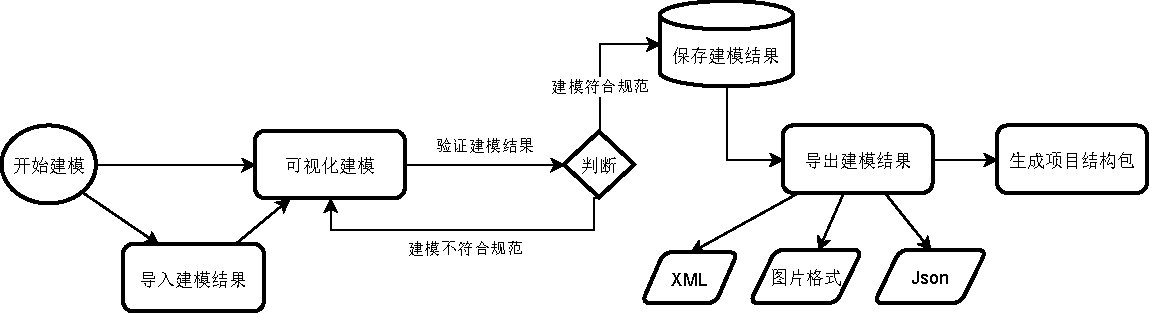
\includegraphics[width=0.8\textwidth]{FIGs/chapter4/toolprocess.pdf} %中括号中的参数是设置图片充满文档的大小,你也可以使用小数来缩小图片的尺寸。
    \caption{建模支持工具业务流程} %caption是用来给图片加上图题的
    \label{toolprocess} %这是添加标签,方便在文章中引用图片。
\end{figure}%figure环境

本章的剩余部分将对建模支持工具进行需求分析,
根据分析得到的结果对工具进行设计与实现。
首先对工具按功能模块进行划分,按模块介绍功能需求与非功能性需求;
然后对工具进行总体设计;最后介绍各模块详细设计与实现。








Finalizer
在一般情况下,如果资源被删除之后,我们虽然能够被触发删除事件,但是这个时候从 Cache 里面无法读取任何被删除对象的信息,这样一来,导致很多垃圾清理工作因为信息不足无法进行,K8s 的 Finalizer 字段用于处理这种情况。在 K8s 中,只要对象 ObjectMeta 里面的 Finalizers 不为空,对该对象的 delete 操作就会转变为 update 操作,具体说就是 update  deletionTimestamp 字段,其意义就是告诉 K8s 的 GC“在deletionTimestamp 这个时刻之后,只要 Finalizers 为空,就立马删除掉该对象”。

所以一般的使用姿势就是在创建对象时把 Finalizers 设置好(任意 string),然后处理 DeletionTimestamp 不为空的 update 操作(实际是 delete),根据 Finalizers 的值执行完所有的 pre-delete hook(此时可以在 Cache 里面读取到被删除对象的任何信息)之后将 Finalizers 置为空即可。

数据卷扩容
https://blog.fleeto.us/post/k8s-1.11-resizing-pvc/
https://cloud.tencent.com/developer/article/1469645
https://www.cnblogs.com/fat-girl-spring/p/15176272.html


最后部署operator的时候
在Kubernetes集群中部署«操作员»时,使用了Helm工具[17]。该工具允许使用一个命令部署应用程序(图6)。我们可以为Helm开发特殊的清单(图表),以表示Kubernetes中的«操作员»应用程序。这些清单包含有关应用程序的所有必要信息,因此Kubernetes可以正确地部署它。例如,我们可以指定应该在Kubernetes集群上部署多少个应用程序副本


基础架构的云独立性,取消对云提供商的依赖

计算资源管理层支持公有云、专有云以及混合云,为区块链服务及上层应用提供所需要的云基础资源。

区块链底层平台是BaaS平台的核心,构建于云容器服务集群之上,支持超级账本、以太坊等不同区块链底层架构。
区块链服务层依托底层区块链的支持,抽象封装一系列服务模块,简化开发工作,帮助企业快速部署区块链应用,降低区块链开发门槛。
管理服务为用户提供基本管理功能,包括平台用户权限管理功能、服务使用计费管理功能、通知功能等。
运维服务提供图形化的区块链管理运维服务能力,实时监控区块链网络运行数据,帮助运维人员及时发现并解决问题。

区块链云化降低开发门槛。区块链技术与其他技术不同之处在于它是融合密码学、P2P网络、分布式存储等多种技术的组合体,技术门槛高致使其开发成本高。而区块链云化产品BaaS平台将区块链技术封装在底层,使功能模块化,开发人员直接调用封装后的API接口即可完成一键部署,降低中小企业用区块链技术的门槛,从而推动区块链应用的落地。

区块链云化实现个性化定制。区块链云化产品BaaS平台可依托云服务商强大的业务能力,在提供标准服务基础上再根据开发者业务需求提供不同的配置,扩展开发者自定义的功能,满足其个性化需求,提高灵活性。同时通过BaaS平台可以沉淀出一层标准的区块链应用解决方案模板,为用户快速匹配建链场景。

市场前景广阔,发展迅速。区块链技术的不断成熟加速了区块链行业应用落地,不断扩大BaaS市场规模,对全球云计算的服务市场促进作用明显。特别是云服务开放性和资源可扩展性使其成为区块链应用落地的最佳载体,区块链与云计算结合愈发紧密。云链协同在加快区块链产业发展的同时,也成为云计算产业发展的关键性新动能。

负责实现云资源的管理调度,该模块会调用云资源管理适配模块的统一接口,所以底层不同云平台接口的差异性对该模块是透明的。该模块的主要功能有创建及删除虚拟机(Docker容器) 和网络资源、进行初始化配置、对已有资源进行扩容或缩容等操作。

对区块链节点的跨云部署支持,需要由该模块来实现对不同公有云、私有云的虚拟机、Docker容器等资源调度API的封装,屏蔽各种云平台API的差异性,对上层调用模块提供统一的资源管理接口。

数据存储
数据存储的核心任务是把数据账本高效地读写到持久化介质中。JD Chain把数据账本模型映射为“键值”结构,为数据的存储提供更好的伸缩性。另外,还定义了标准的持久化服务SPI,能够适配不同的数据库引擎,更好地复用企业现有的IT基础设施,满足企业的多样化需求。

华为云区块链服务基于可信、开放、服务全球的华为云上运行,华为云产品和服务具有华为独有的新技术,以降低成本、弹性灵活、电信级安全、高效自助管理等优势惠及用户,BCS 可以和华为云技术产品和行业解决方案无缝对接,帮助企业在安全、高效、不可篡改等基础上轻松跨入云时代,快速部署新解决方案和应用。

本文还实现了基于Hyperledger Fabric的云化工具

为解决上述挑战, 本文
Hyperledger Fabric Operator: 云原生时代下Fabric管理工具
利用Kubernetes,72\%的工程师在云原生生产中使用Kubernetes[3],可以方便的迁移到支持Kubernetes的任何云 
更简单、更原生的: 使用kubectl命令管理Fabric, 显示于k8s-dashboard;复用Kubernetes, API公共功能如CRUD、watch、内置认证
管理Fabric: 声明式自动化配置静态组件,如: CA、HF网络组件.命令式创建动态通道、链码

由linux基金会牵头,包括 IBM等30家初始企业成员共同成立的Hyperledger Fabric项目成为流行的面向联盟链场景开源框架之一。该项目定位是面向企业的分布式账本平台,引入权限管理,设计上支持可插拔、可扩展,自开源依赖广受欢迎,github上已经有12.7k star。然而云原生时代下,Fabric缺乏一个成熟的、一站式的解决方案来解决在云计算平台上构建区块链联盟链(私有链)。

区块链作为一种点对点的信息和价值交换的“桥梁”,通过定义一套标准的操作接口和数据结构,能够提升多方业务对接的效率,降低应用落地的复杂度。遵循标准化原则,要求在系统设计时数据模型及操作模型独立于系统实现,让数据“系于链却独于链”,可在链下被独立地验证和运用,更好地支持企业进行数据治理,提升区块链系统的灵活性和通用性




\section{需求分析}

\subsection{工具总体功能}

DDDD(Draw for Domain-Driven Design)建模支持工具总体功能规划
如图\ref{toolstotal}所示,
主要包括“可视化建模”模块、“模型校验”模块以及“模型存储与转化”模块,
各模块详细功能需求描述如下:

\begin{figure}[!htbp] %figure环境,h默认参数是可以浮动,不是固定在当前位置。如果要不浮动,你就可以使用大写float宏包的H参数,固定图片在当前位置,禁止浮动。
    \centering %使图片居中显示
    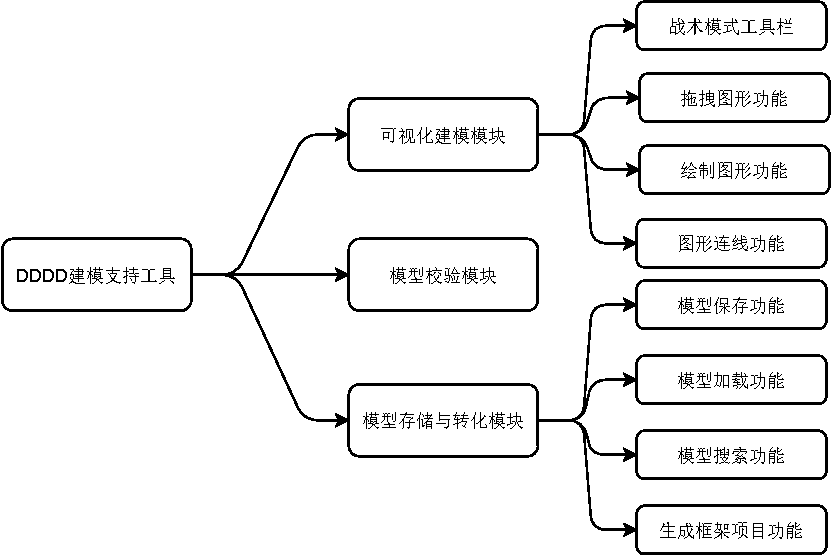
\includegraphics[width=0.8\textwidth]{FIGs/chapter4/toolstotal.pdf} %中括号中的参数是设置图片充满文档的大小,你也可以使用小数来缩小图片的尺寸。
    \caption{工具总体功能} %caption是用来给图片加上图题的
    \label{toolstotal} %这是添加标签,方便在文章中引用图片。
\end{figure}%figure环境


% \begin{figure}[!htbp] %figure环境,h默认参数是可以浮动,不是固定在当前位置。如果要不浮动,你就可以使用大写float宏包的H参数,固定图片在当前位置,禁止浮动。
%     \centering %使图片居中显示
%     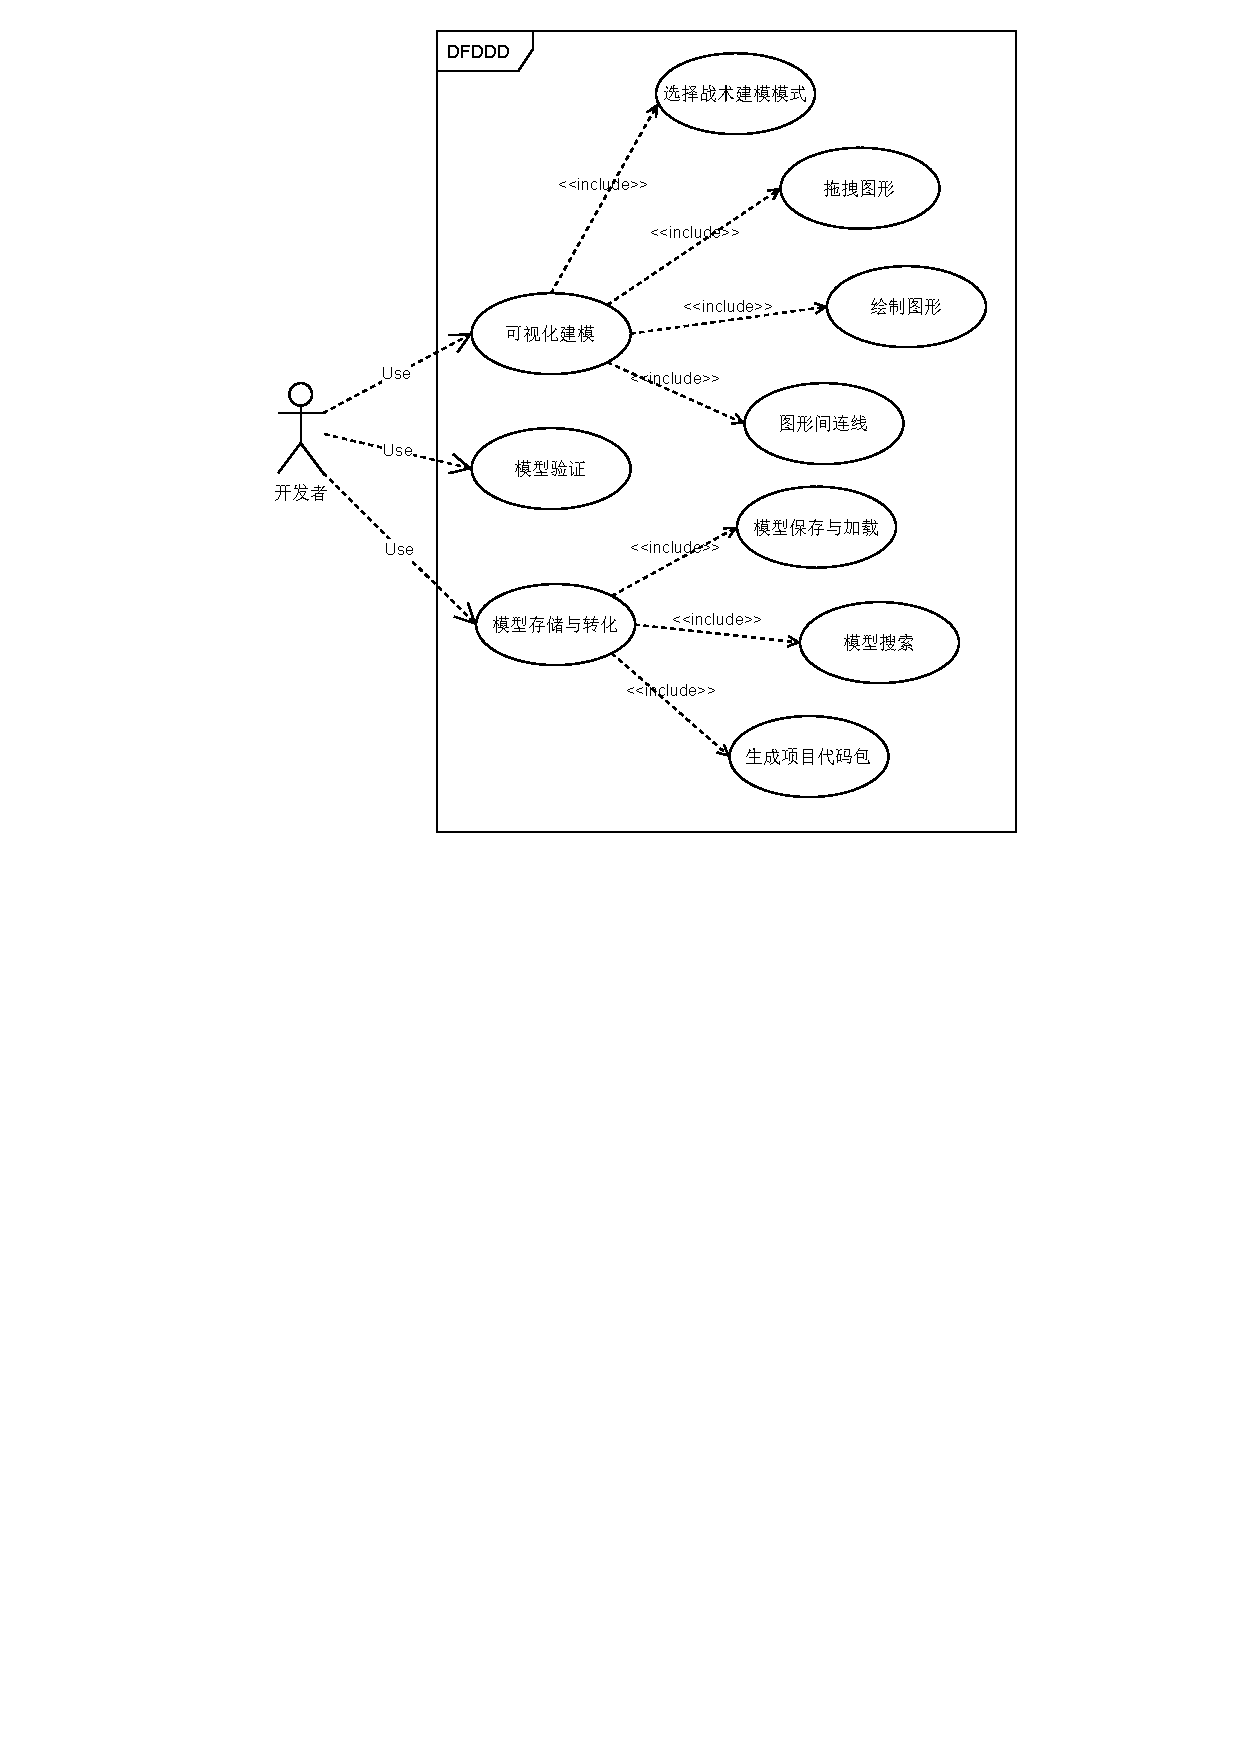
\includegraphics[width=0.8\textwidth]{FIGs/chapter4/usecaseDFDDD.pdf} %中括号中的参数是设置图片充满文档的大小,你也可以使用小数来缩小图片的尺寸。
%     \caption{建模支持工具用例图} %caption是用来给图片加上图题的
%     \label{usecaseDFDDD} %这是添加标签,方便在文章中引用图片。
% \end{figure}%figure环境

\begin{itemize}
    \item “可视化建模”模块:支持开发人员从工具栏中选择需要使用的战术模式,并灵活地将
    模式图形拖拽到建模绘图面板上进行绘制,还支持根据建模需要对不同的模式进行连线,
    表达模式间的关系,完成可视化建模过程。
    \item “模型校验”模块:在建模过程中或建模完成时,可以依据定义的战术建模元模型中的约束
    对建模的结果进行验证,并给出修改意见。
    \item “模型存储与转化”模块:建模完成后,将建模结果进行存储或导出到本地,
    也可以从数据库或本地读取模型文件,根据建模结果,生成符合领域驱动设计规范的框架项目代码包。

\end{itemize}

\subsection{可视化建模模块需求分析}

\textbf{功能性需求}

“可视化建模”模块是本建模支持工具的核心功能模块,
如图\ref{us1}所示,
开发人员或架构师可以通过“可视化建模”模块“选择战术建模模式”、“拖拽图形”、
“绘制图形”以及进行“图形间连线”。

\begin{figure}[!htbp] %figure环境,h默认参数是可以浮动,不是固定在当前位置。如果要不浮动,你就可以使用大写float宏包的H参数,固定图片在当前位置,禁止浮动。
    \centering %使图片居中显示
    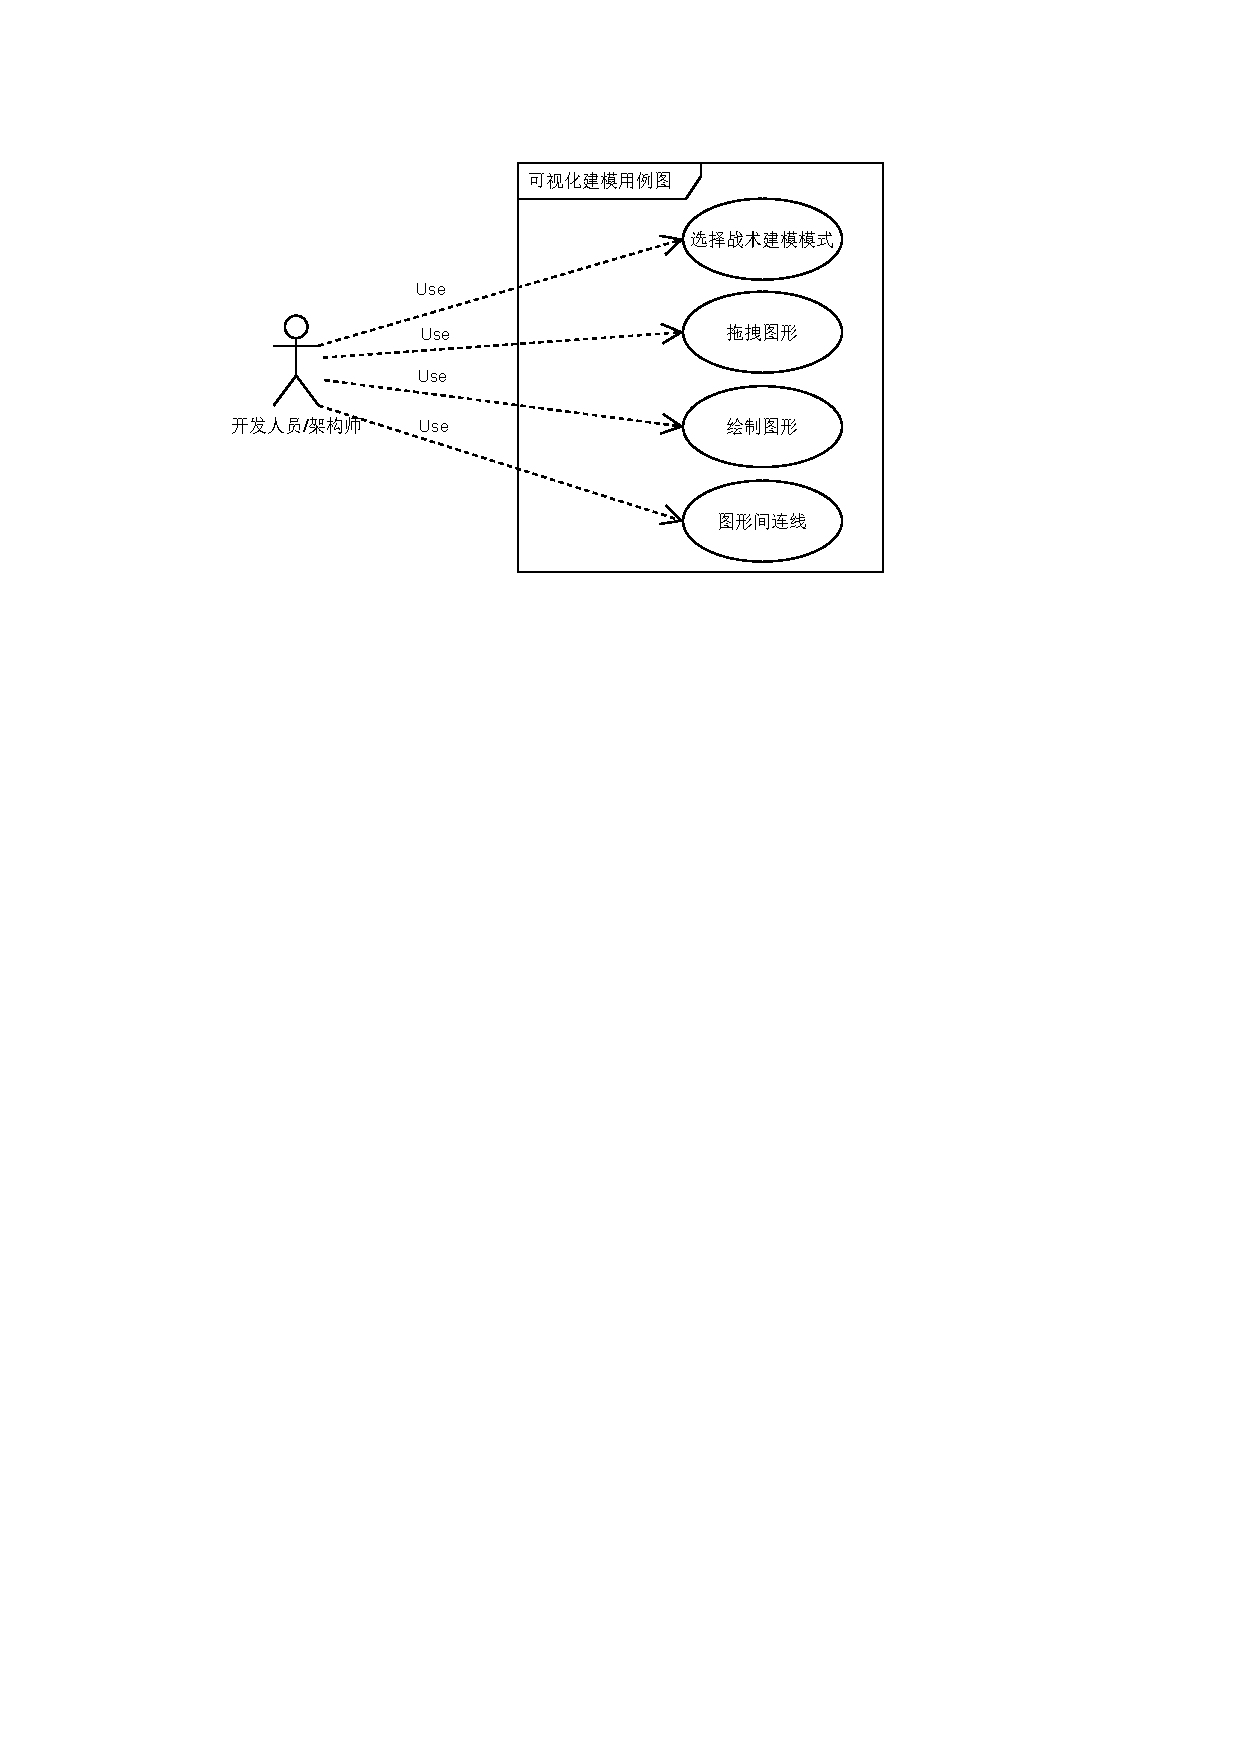
\includegraphics[width=0.8\textwidth]{FIGs/chapter4/us1.pdf} %中括号中的参数是设置图片充满文档的大小,你也可以使用小数来缩小图片的尺寸。
    \caption{可视化建模模块用例图} %caption是用来给图片加上图题的
    \label{us1} %这是添加标签,方便在文章中引用图片。
\end{figure}%figure环境

表\ref{usecase1}展示了“可视化建模”模块的用例描述,
“可视化建模”为开发者提供灵活方便的可拖拽式建模方式,
可以自由选择需要使用的战术模式,拖拽到绘制面板中进行绘制,
对绘制的模型对象可以双击修改文字信息,并将当前模型对象与其他对象进行连线,
以表示它们之间的关系,在绘制面板上方还有以按钮形式提供的绘图操作菜单。

{\footnotesize
\begin{longtable}[h]{m{80pt}|m{305pt}}
    \caption[可视化建模用例表]{可视化建模用例表} \label{usecase1} \\
        \hline  
        ID&UC1\\
        \hline
        名称&可视化建模用例\\
        \hline
        描述&开发者使用工具可以拖拽式地进行建模,选择战术模式相应图形化模型,
        拖拽到建模绘制面板中,并修改模型对象信息、对象间关系,达到灵活可视化建模。\\
        \hline
        触发条件&从主页点击“开始建模”按钮\\
        \hline
        前置条件&用户浏览器支持JavaScript\\
        \hline
        后置条件&无\\
        \hline
        正常流程& (1)用户点击“开始建模”按钮;
        \newline (2)用户点击展开战术模式列表,拖拽需要的模式进入绘图面板;
        \newline (3)松开鼠标,模型对象绘制完成,双击模型对象文字块,修改文字信息;
        \newline (4)当鼠标悬停在模型对象上且边框变绿,按住鼠标左键拖动绘制箭头,
                    连接到其他模型对象上;
        \newline (5)点击绘图板上方按钮可对模型进行验证、组合、分解、删除、撤销以及缩放画布操作。\\
        \hline
        异常流程&无\\
        \hline
    \end{longtable} 
}

\textbf{非功能性需求}

“可视化建模”模块的非功能性需求主要包括易用性、可靠性和可扩展性,
具体需求如下:

\begin{itemize}
    \item 易用性:可视化的建模过程易于学习和使用,
    用户仅需进行简单的拖拉拽操作即可完成图形化建模,
    速度快,图形变换灵活简单,建模结果清晰明确,符合用户建模的期望。

    \item 可靠性:在“可视化建模”过程中,绘图逻辑大多都在前端完成,
     即使网络连接断开也不影响建模过程,保障了建模过程的连贯性。
   
     \item 可扩展性:“可视化建模”的战术模式工具栏可以根据需求添加和删除战术模式,
     适应未来战术建模理论的更新和发展。
\end{itemize}

\subsection{模型校验模块需求分析}

\textbf{功能性需求}

“模型校验”模块用例图如图\ref{us2}所示,
该模块帮助开发人员或架构师根据元模型和约束规则对建模结果进行验证和修改。

表\ref{usecase2}展示了"模型校验"功能模块的用例描述,
“模型校验”根据本文定义的战术建模元模型约束规则和图形绘制规则对图形化的建模结果
进行验证,对不符合规范和约束的模型进行警告和给出修改提示,
对验证通过的模型进行命名并保存到数据库中。

\begin{figure}[!htbp] %figure环境,h默认参数是可以浮动,不是固定在当前位置。如果要不浮动,你就可以使用大写float宏包的H参数,固定图片在当前位置,禁止浮动。
    \centering %使图片居中显示
    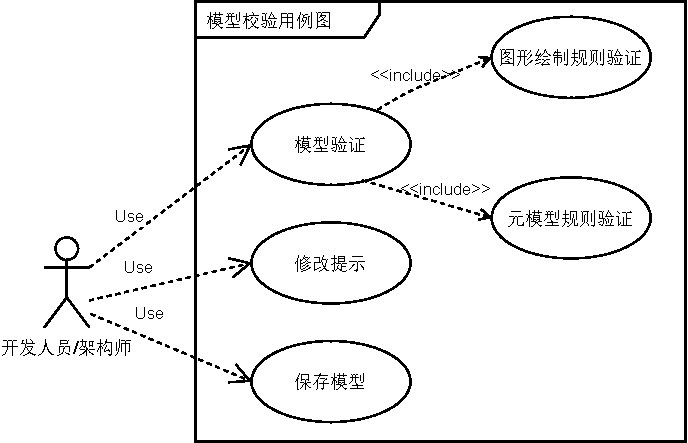
\includegraphics[width=0.8\textwidth]{FIGs/chapter4/us2.pdf} %中括号中的参数是设置图片充满文档的大小,你也可以使用小数来缩小图片的尺寸。
    \caption{模型校验模块用例图} %caption是用来给图片加上图题的
    \label{us2} %这是添加标签,方便在文章中引用图片。
\end{figure}%figure环境


{\footnotesize
\begin{longtable}[h]{m{80pt}|m{305pt}}
    \caption[模型校验用例表]{模型校验用例表} \label{usecase2} \\
        \hline  
        ID&UC2\\
        \hline
        名称&模型校验\\
        \hline
        描述&根据本文提出的战术建模元模型及约束规则对建模结果进行验证,
        并给出修改意见\\
        \hline
        触发条件&绘图界面点击“验证”按钮\\
        \hline
        前置条件&建模进行中或已经完成\\
        \hline
        后置条件&无\\
        \hline
        正常流程& (1)当建模面板不为空时,开发者点击“验证”按钮;
        \newline (2)前端界面弹出验证通过或验证失败及修改提示信息;
        \newline (3)如果验证通过,将建模结果命名并自动保存在数据库中。\\
        \hline
        异常流程&保存建模结果时未填写名称,提示填写\\
        \hline
    \end{longtable} 
}

\textbf{非功能性需求}

“模型校验”模块的非功能性需求主要包括易用性、健壮性和可靠性,
具体需求如下:

\begin{itemize}
    \item 易用性:模型的验证结果以弹窗形式展示,
    指出建模不规范的地方并给出修改建议,
    让用户明确需要修改哪些建模结果。

    \item 健壮性:验证操作能够应对各种异常情况并作出响应。
    对于错误输入、非法字符和误操作等能够规避和纠正,
    有效防止建模过程中工具的崩溃。
   
     \item 可靠性:支持每次验证操作都将建模结果自动保存到数据库,
    保障了建模结果不丢失和及时更新持久化内容。
\end{itemize}

\subsection{模型存储与转化模块需求分析}

“模型存储与转化”模块用例图如图\ref{us3}所示,
开发人员或架构师通过“模型存储与转化”模块对模型进行导入和导出,
对数据库中存储的模型进行管理,即搜索和查看模型,还能根据模型生成框架项目。

\begin{figure}[h] %figure环境,h默认参数是可以浮动,不是固定在当前位置。如果要不浮动,你就可以使用大写float宏包的H参数,固定图片在当前位置,禁止浮动。
    \centering %使图片居中显示
    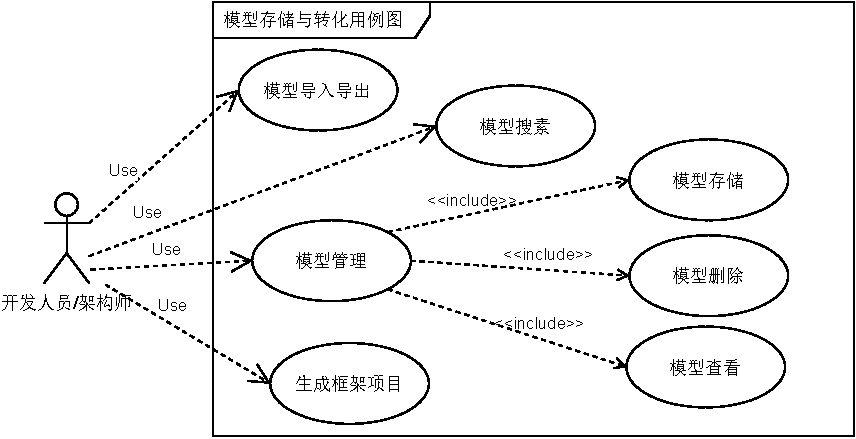
\includegraphics[width=0.8\textwidth]{FIGs/chapter4/us3.pdf} %中括号中的参数是设置图片充满文档的大小,你也可以使用小数来缩小图片的尺寸。
    \caption{模型存储与转化模块用例图} %caption是用来给图片加上图题的
    \label{us3} %这是添加标签,方便在文章中引用图片。
\end{figure}%figure环境

表\ref{usecase3}展示了“模型存储与转化”模块的用例描述,
“模型管理”可以将通过验证的建模结果保存到数据库中,
“模型导入导出”可以将模型以XML、图片等文件格式导出到本地,
也可以导入本地模型文件或搜索数据库中现有模型进行展示和修改,
通过“生成框架项目”可以得到符合领域驱动设计规范的框架项目代码包。

{\footnotesize
    \begin{longtable}[h]{m{80pt}|m{305pt}}
        \caption[模型存储与转化用例表]{模型存储与转化用例表} \label{usecase3} \\
            \hline  
            ID&UC3\\
            \hline
            名称&模型存储与转化\\
            \hline
            描述&将图形化建模结果存储到数据库,或直接以XML、图形等格式导出到本地,
            也可以从本地导入XML模型文件,根据完整的建模结果,自动生成符合领域驱动设计
            结构规范的框架项目代码\\
            \hline
            触发条件&绘图界面点击“导入”、“导出”、“验证”、“保存”或“生成项目”按钮\\
            \hline
            前置条件&建模进行中或已经完成\\
            \hline
            后置条件&无\\
            \hline
            正常流程& (1)进入绘图界面时,可以选择导入本地模型文件或搜索数据库中模型文件进行继续建模;
            \newline (2)模型验证通过后,选择导出建模结果到本地或存储到数据库中;
            \newline (3)点击绘图面板上方“生成项目”按钮可以生成框架项目文件。\\
            \hline
            异常流程&保存建模结果时未填写名称,提示填写\\
            \hline
        \end{longtable} 
}

\textbf{非功能性需求}

“模型存储与转化”模块的非功能性需求主要包括可扩展性、可靠性和性能,
具体需求如下:
        
        \begin{itemize}
            \item 可扩展性:工具采用前后端分离的结构,
            可以对前端或后端组件进行替换或扩展。
            满足存储持久化设施多样性,
            为后续存储更多模型提供保障。
        
            \item 可靠性:工具支持本地文件系统的导入导出,
            不强依赖远程数据库,满足各种网络条件下的建模需求。
           
             \item 性能:对于数据存储和检索使用了ElasticSearch,
             基于倒排索引能达到高效的全文搜索\cite{divya2013elasticsearch}。
             满足搜索模型的即时性,让工具使用速度提升。
        \end{itemize}

\section{工具设计与实现}
\subsection{总体设计}


% 支持建模方法的工具使用流程如下图\ref{toolprocess}所示。
% 开发者使用支持工具开始建模,首先可以选择学习或回顾DDD基本概念知识,
% 为后续建模做理论准备,也可以继续从上一次建模保存的结果开始继续建模;
% 进行可视化建模时,开发者可以随时进行对建模结果的验证,
% 工具将对不符合规范的建模结果给出提示和警告;如果建模结果符合规范和约束,
% 工具将保存建模结果到数据库,通过工具可以将建模结果以XML、图片或Json格式导出;
% 最后,还可以根据建模结果生成框架项目文件。

本工具的架构根据典型的四层架构\cite{王君2007基于}进行设计和划分,
整体架构图如图\ref{overallarchitecture}所示。
第一层表现层负责向用户展示业务流程和数据,包含可视化建模
与验证修改模型等功能;第二层服务层,包含对模型的
存储以及读取、对模型的二次校验和框架项目文件生成功能;
第三层持久层主要保存了业务模型对象的数据,
即对实体、值对象和领域服务等对象数据进行保存;
第四层数据层主要负责建模结果的保存和读取。

\begin{figure}[!htbp] %figure环境,h默认参数是可以浮动,不是固定在当前位置。如果要不浮动,你就可以使用大写float宏包的H参数,固定图片在当前位置,禁止浮动。
    \centering %使图片居中显示
    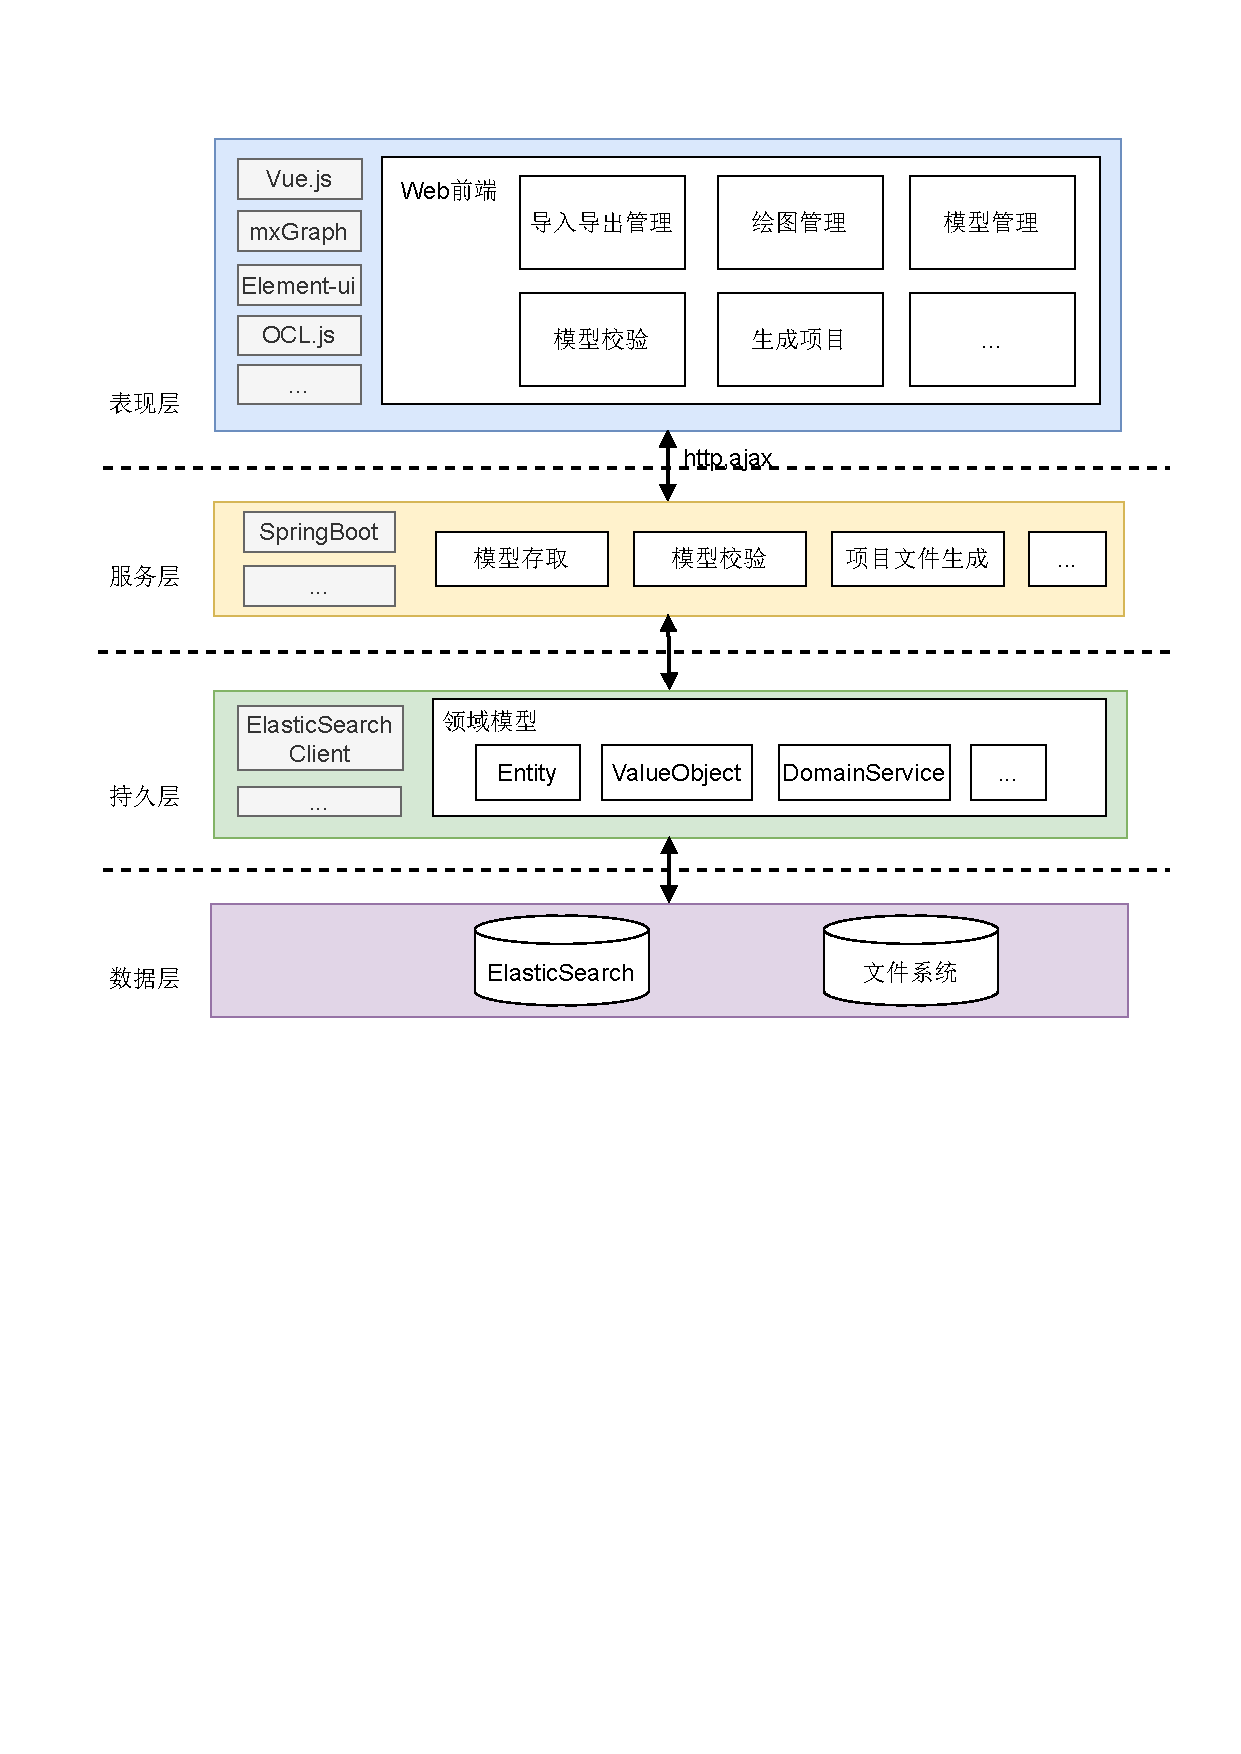
\includegraphics[width=0.8\textwidth]{FIGs/chapter4/overallarchitecture.pdf} %中括号中的参数是设置图片充满文档的大小,你也可以使用小数来缩小图片的尺寸。
    \caption{支持工具整体架构图} %caption是用来给图片加上图题的
    \label{overallarchitecture} %这是添加标签,方便在文章中引用图片。
\end{figure}%figure环境


\begin{itemize}
    \item 表现层:该层为用户提供访问入口,通过该层用户可以直观地使用
    “可视化建模”、”模型校验“等工具核心功能。工具前端采用Vue.js框架
    结合ElementUI组件进行开发,使整个页面整洁美观,交互良好;对于
    图形的拖拽和绘制,采用开源框架mxGraph作为底层支持,mxGraph拥有
    优秀的交互和卓越的性能,已经在许多商业软件中被使用,能有效支持灵活的
    图形编辑;OCL.js主要用来支持模型规范和标准的校验,充当对象约束语言和
    前端JavaScript之间的媒介,可以直接使用JavaScript完成OCL的功能。
    \item 服务层:该层主要提供后端接口服务和对建模逻辑的二次验证。
    后端整体采用Spring Boot框架进行开发,封装抽象了核心的业务逻辑模型(实体、值对象等),
    提供了模型存取与框架项目文件生成的业务逻辑。
    \item 持久层:该层主要充当数据层与服务层间交互的媒介,将业务逻辑模型
    对象转化为底层数据。持久化存储采用ElasticSearch Client与数据层进行
    通信,通过RESTful接口进行写入和读取。
    \item 数据层:该层是底层的存储数据依赖,模型底层存储格式为XML文件,
    文件篇幅较长,但对读写并发要求不高。采用两种数据基础设施进行实现,
    采用ElasticSearch支持大篇幅文档型数据存储,提高模型搜索的检索效率,
    也可根据用户需要直接存储到本地文件系统。
\end{itemize}

建模支持工具DDDD是一个前后端分离的Web应用。前端采用mxGraph结合Vue.js
进行开发实现,后端采用Spring Boot框架,以ElasticSearch作为持久化机制
进行实现,前后端采用RESTful风格进行交互\cite{richardson2008restful}。

由于建模过程的可视化描述和模型校验反馈是工具的核心内容,
负责与用户交互和展示模型的Web前端的架构也有一定复杂度,
故采用如图\ref{frontarchitecture}所描述的整洁架构\cite{martin2018clean}对前端进行划分。
整洁架构是一种与数据库、客户端接口以及框架都无关的架构,
可以用来构建复杂的前端项目,将业务逻辑抽离,但又不依赖后端,保证项目的可扩展性。
本工具使用整洁架构将前端划分为三层,包括表现层、领域层和数据层。
表现层包含绘图、校验、导入导出以及菜单等与用户交互的模块;
领域层包含展示模型和校验反馈的底层业务逻辑,如拖拽绘制、
校验模型、导入导出模型、画布管理、路由管理以及生成项目等功能;
数据层包含调用后端API连接的远程数据源和本地数据源,
负责存储和获取模型。

\begin{figure}[htb] %figure环境,h默认参数是可以浮动,不是固定在当前位置。如果要不浮动,你就可以使用大写float宏包的H参数,固定图片在当前位置,禁止浮动。
    \centering %使图片居中显示
    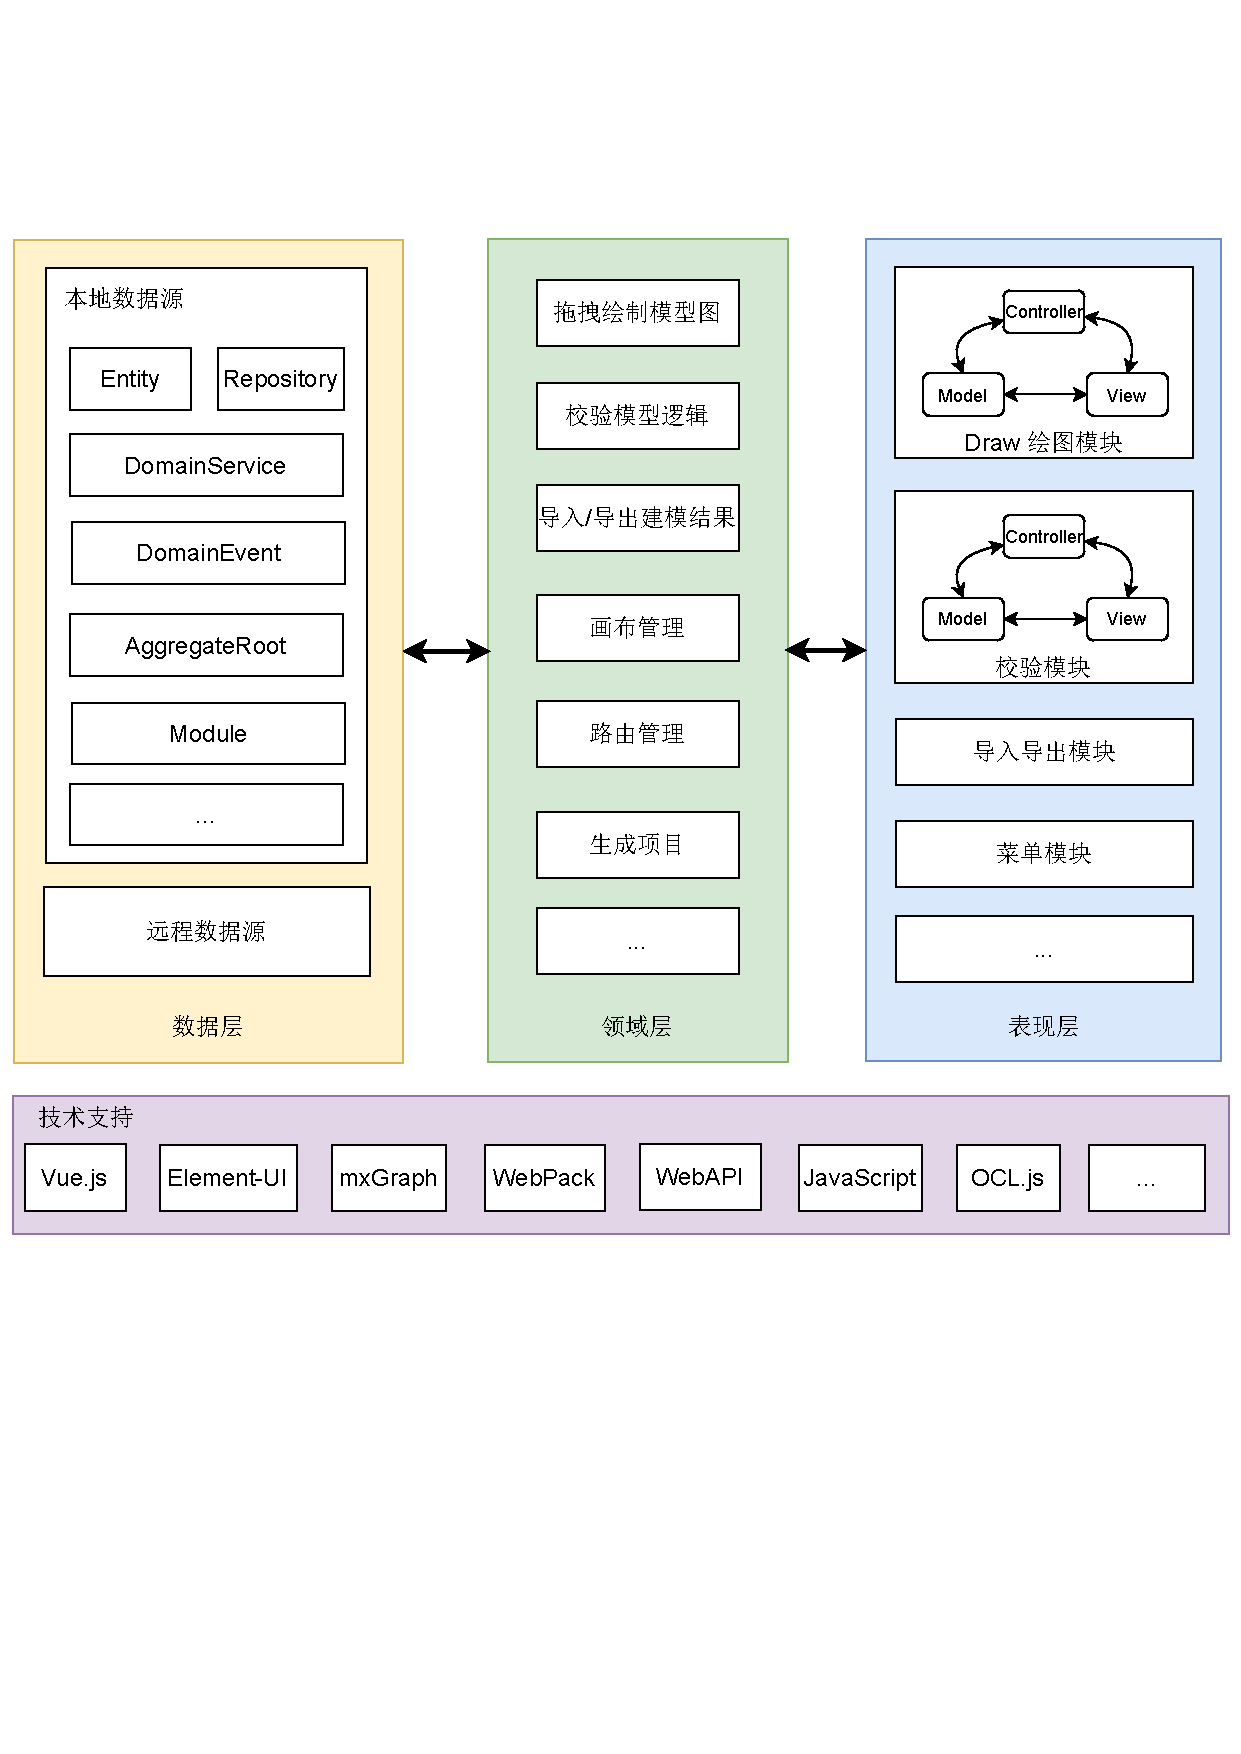
\includegraphics[width=0.8\textwidth]{FIGs/chapter4/frontarchitecture.pdf} %中括号中的参数是设置图片充满文档的大小,你也可以使用小数来缩小图片的尺寸。
    \caption{支持工具前端整洁架构图} %caption是用来给图片加上图题的
    \label{frontarchitecture} %这是添加标签,方便在文章中引用图片。
\end{figure}%figure环境


\subsection{可视化建模模块详细设计与实现}

本小节将介绍“可视化建模”模块的详细设计与实现。详细设计部分,
通过类图展现“可视化建模”模块的静态详细设计,
通过顺序图展现“可视化建模”模块的动态业务流程详细设计。
实现部分,通过部分核心功能的实现代码来进行展现。
“可视化建模”模块具体的设计如下:

\textbf{可视化建模类图}

“可视化建模”模块类图如图\ref{classDrawVisualization}所示。
本工具提供对建模过程可视化的支持,主要由Canvas类对mxGraph中
封装好的画图工具类接口进行调用,并确保工具类是单例的,
Canvas类还负责工具运行时对画布的初始化,保证画图时的线条、箭头和颜色
符合预期,最后,还包含绘制新图形时的判断逻辑。Toolbar类主要
提供了建模时对模式的选择支持,可以直接从中点击拖动实现选择战术模式。
Menu类包含了对画布操作的一系列接口。
Container类负责统一管理Toolbar、Canvas和Menu类,并收集反馈信息与用户进行交互。

\begin{figure}[!htbp] %figure环境,h默认参数是可以浮动,不是固定在当前位置。如果要不浮动,你就可以使用大写float宏包的H参数,固定图片在当前位置,禁止浮动。
    \centering %使图片居中显示
    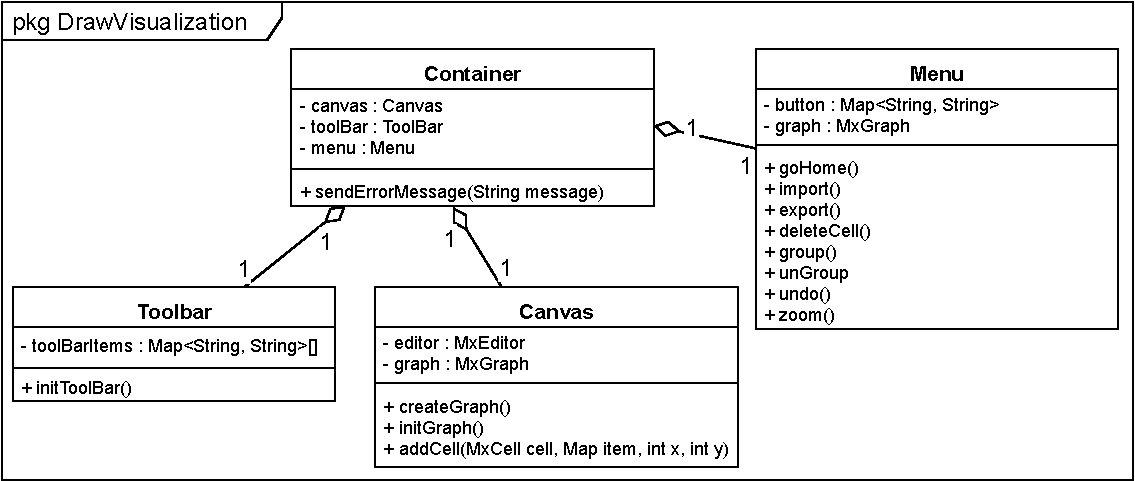
\includegraphics[width=0.8\textwidth]{FIGs/chapter4/classDrawVisualization.pdf} %中括号中的参数是设置图片充满文档的大小,你也可以使用小数来缩小图片的尺寸。
    \caption{可视化建模模块类图} %caption是用来给图片加上图题的
    \label{classDrawVisualization} %这是添加标签,方便在文章中引用图片。
\end{figure}%figure环境

\textbf{可视化建模顺序图}

“可视化建模”模块的示例过程如图\ref{sdDrawVisualization}所示。
首先开发人员或架构师通过使用Container类初始化画布、工具栏等可视化建模必要元素,
通过Toolbar类实现拖拽图形化模式对象,并在合适的位置由Canvas类绘制,
在建模过程中,通过菜单可以实现撤销、重做、组合、删除、缩放画布等一系列操作,
辅助完成建模过程,在建模过程中画布会实时反馈信息给用户。

\begin{figure}[!htbp] %figure环境,h默认参数是可以浮动,不是固定在当前位置。如果要不浮动,你就可以使用大写float宏包的H参数,固定图片在当前位置,禁止浮动。
    \centering %使图片居中显示
    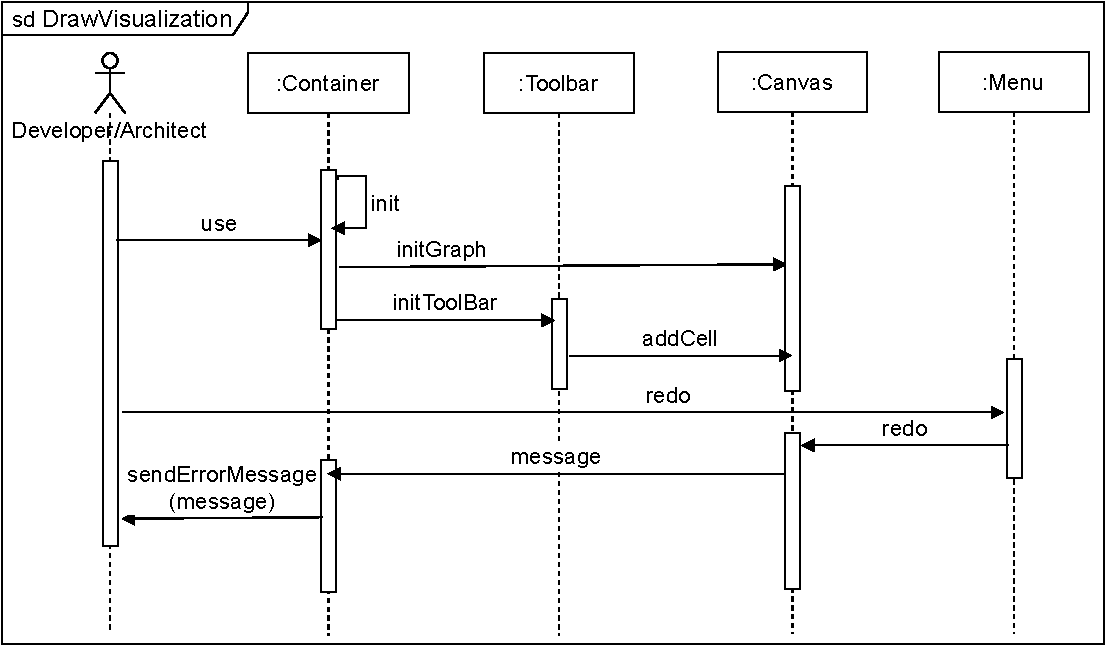
\includegraphics[width=0.8\textwidth]{FIGs/chapter4/sdDrawVisualization.pdf} %中括号中的参数是设置图片充满文档的大小,你也可以使用小数来缩小图片的尺寸。
    \caption{可视化建模模块顺序图} %caption是用来给图片加上图题的
    \label{sdDrawVisualization} %这是添加标签,方便在文章中引用图片。
\end{figure}%figure环境

\newpage
\textbf{可视化建模实现代码}

如图\ref{initToolbar}所示为“可视化建模”核心功能工具栏的初始化代码。
代码描述了获取图形对象数组、拖动图形、绘制图形的逻辑。

\begin{figure}[!htbp] %figure环境,h默认参数是可以浮动,不是固定在当前位置。如果要不浮动,你就可以使用大写float宏包的H参数,固定图片在当前位置,禁止浮动。
    \centering %使图片居中显示
    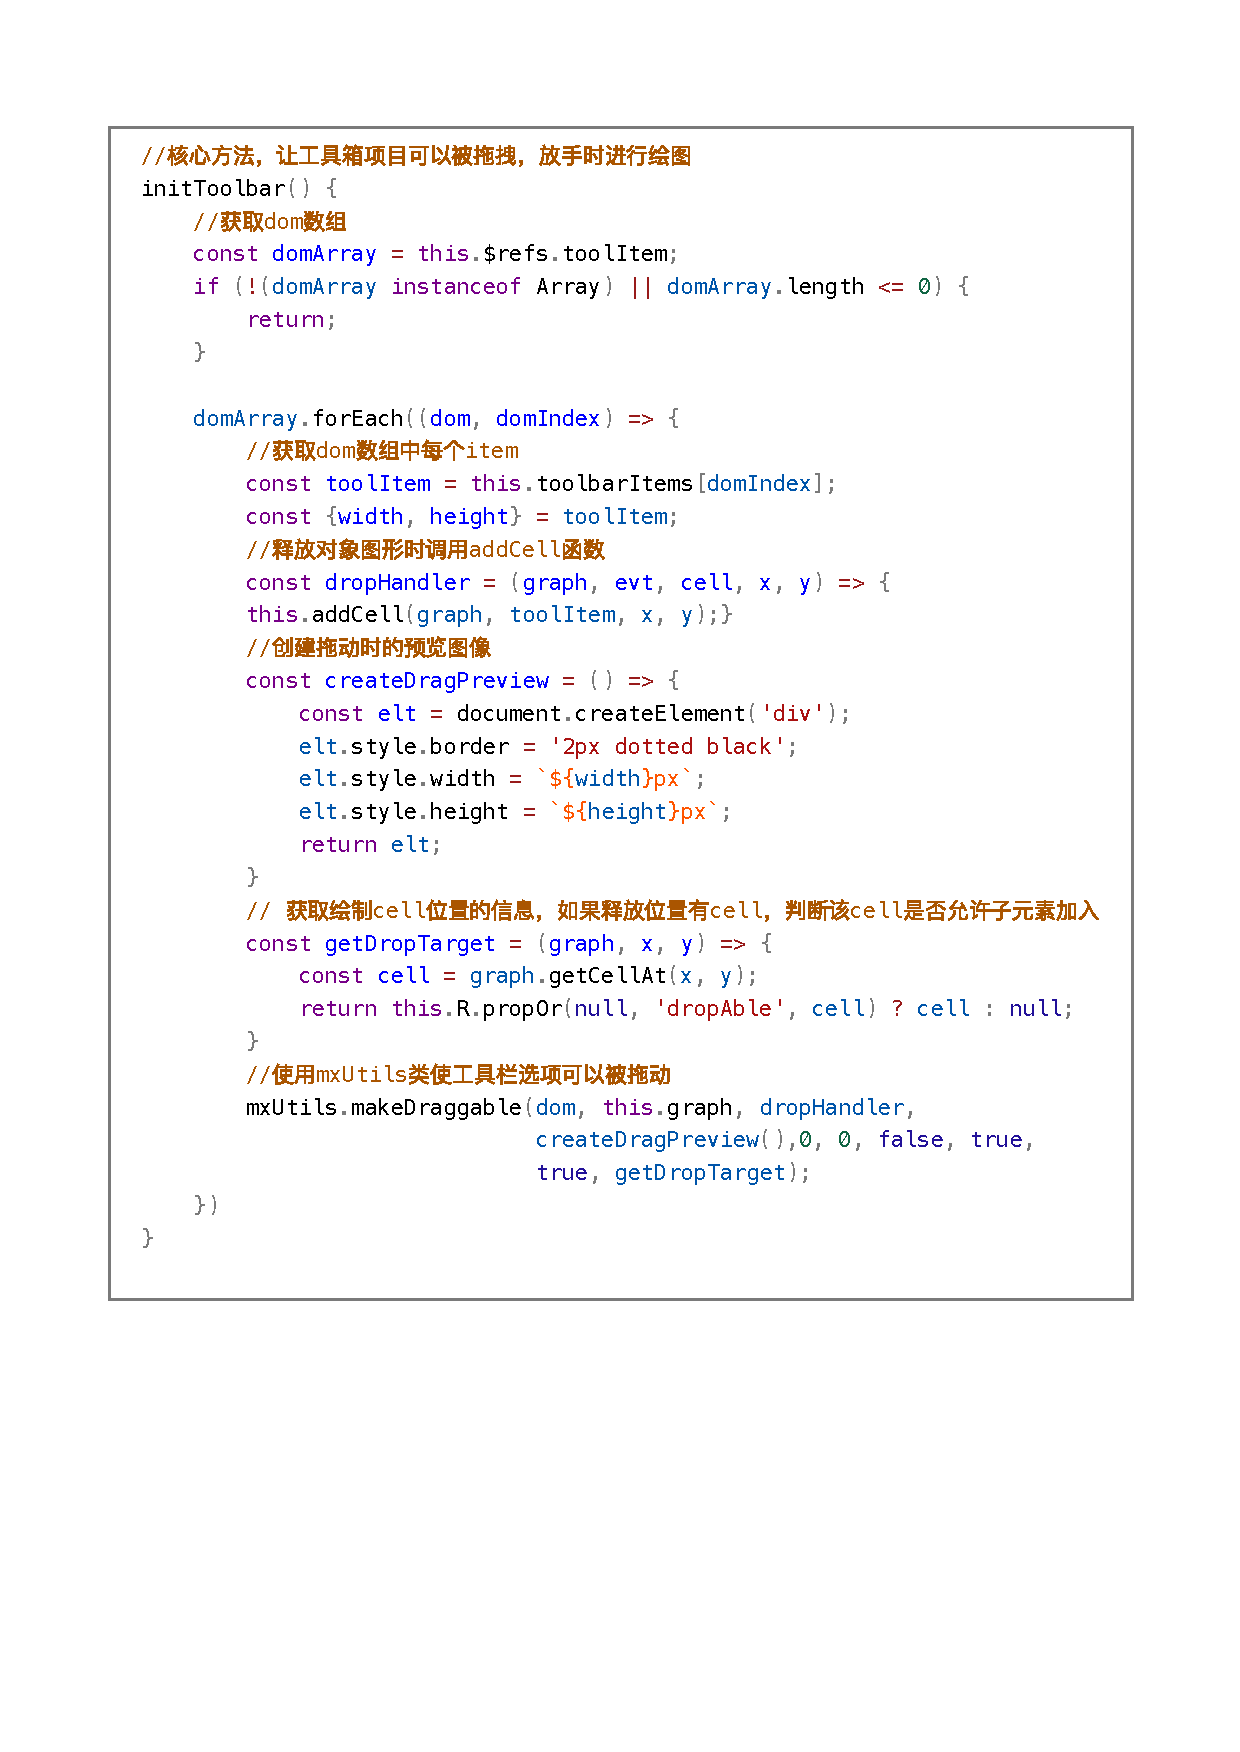
\includegraphics[width=0.8\textwidth]{FIGs/chapter4/initToolbar.pdf} %中括号中的参数是设置图片充满文档的大小,你也可以使用小数来缩小图片的尺寸。
    \caption{初始化ToolBar代码} %caption是用来给图片加上图题的
    \label{initToolbar} %这是添加标签,方便在文章中引用图片。
\end{figure}%figure环境 

\subsection{模型校验模块详细设计与实现}

本小节将介绍“模型校验”模块的详细设计与实现。详细设计部分,
通过类图展现“模型校验”模块中各战术模式的静态详细设计;
实现部分,
通过校验算法展现“模型校验”模块的验证逻辑的设计,
通过部分实现代码展示具体实现。
“模型校验”模块具体的设计如下:

\newpage
\textbf{模型校验类图}

“模型校验”模块类图如图\ref{classValidation}所示。
本工具提供对建模结果的校验,战术模式统一继承自Pattern类,
Pattern类描述了模式的名称、类型、连接输入以及连接输出,
并在validation方法中调用OCLEngine对象实例完成对象约束语言的验证。
PatternData用来记录所有Pattern子类实例的数据细节,
辅助校验过程。


\begin{figure}[!htbp] %figure环境,h默认参数是可以浮动,不是固定在当前位置。如果要不浮动,你就可以使用大写float宏包的H参数,固定图片在当前位置,禁止浮动。
    \centering %使图片居中显示
    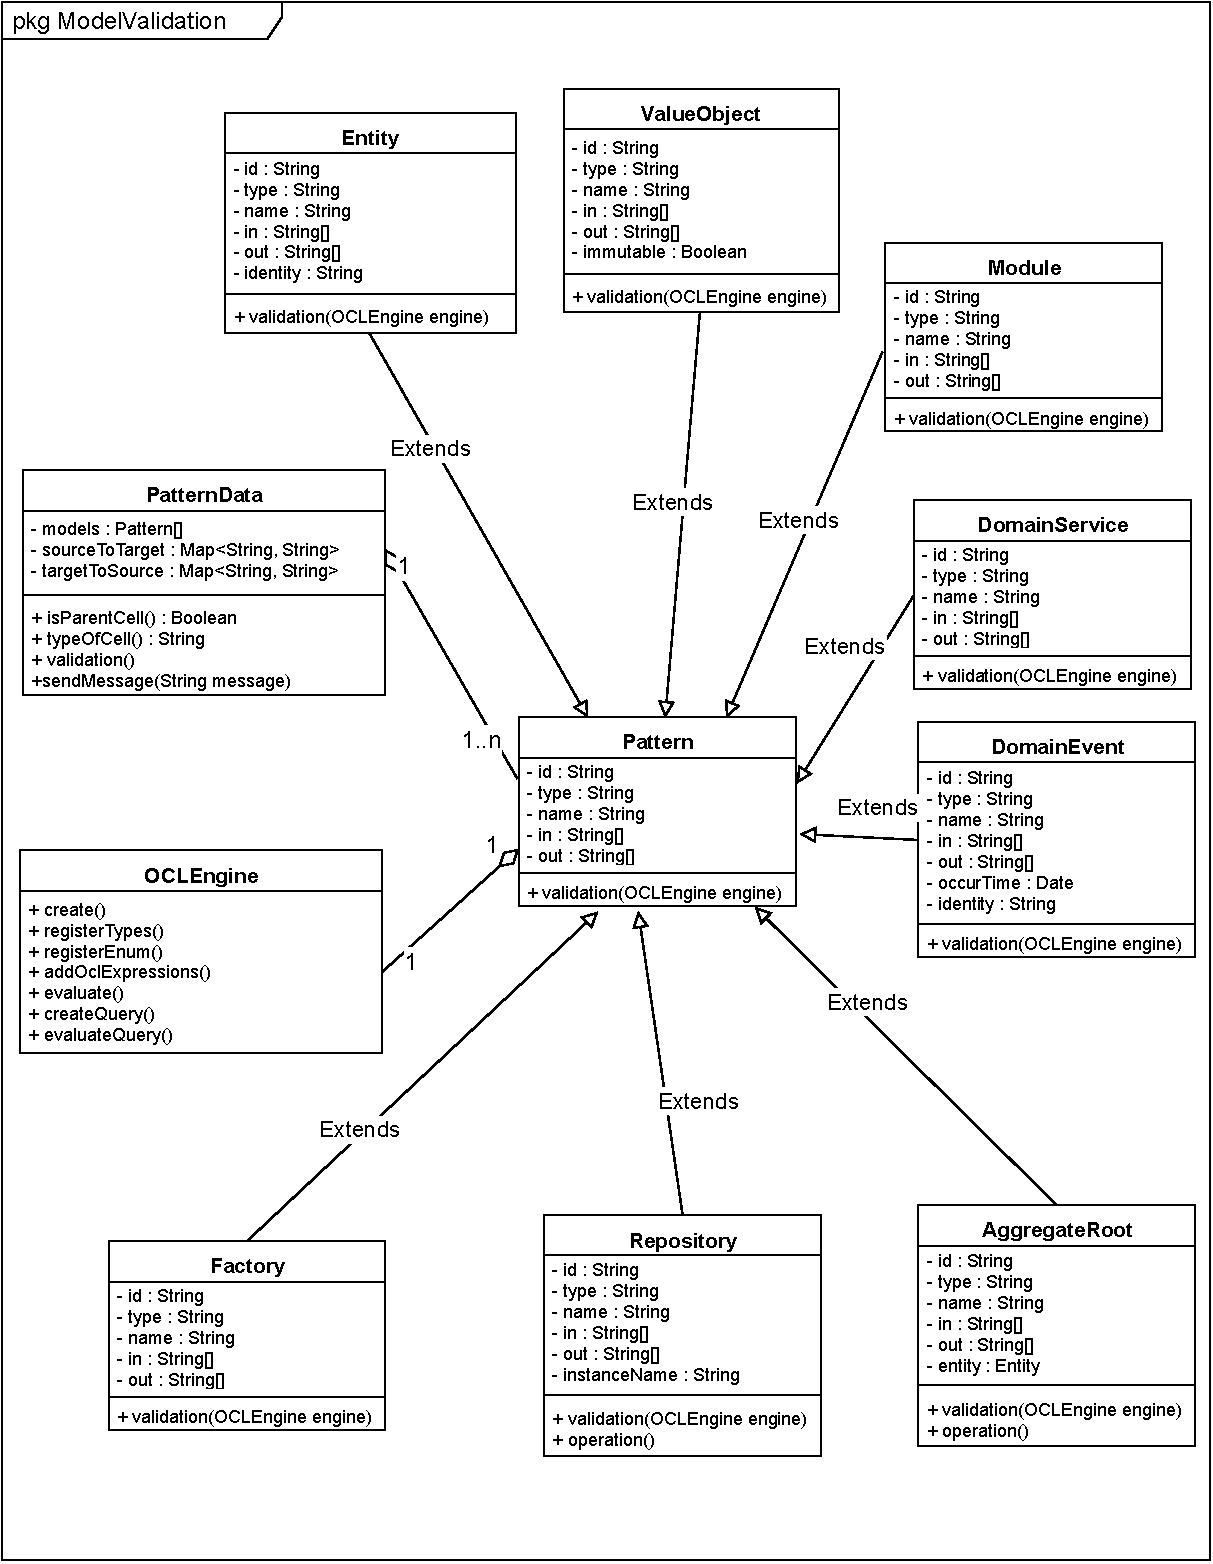
\includegraphics[width=0.8\textwidth]{FIGs/chapter4/classValidation.pdf} %中括号中的参数是设置图片充满文档的大小,你也可以使用小数来缩小图片的尺寸。
    \caption{模型校验模块类图} %caption是用来给图片加上图题的
    \label{classValidation} %这是添加标签,方便在文章中引用图片。
\end{figure}%figure环境

\textbf{模型校验算法}

“模型校验”功能的具体实现逻辑如算法\ref{algorithm1}所示。该算法首先通过遍历所有图形化对象节点,
建立两种连接关系双向映射,第一种描述源对象到目标对象映射关系,第二种描述目标对象到源对象映射关系;
然后进行第二次遍历,首先判断该对象节点是否为顶级节点,只有顶级节点才作为战术模式元素,
如果为顶级节点,则调用PatternData类中的validation函数进行模式属性以及OCL约束验证,
验证通过将该对象以具体模式(实体、值对象等)添加到patternData的models数据结构中,若验证失败,
将布尔型成功标识变量标记为否,并退出循环体。无论验证是否通过,都将非顶级节点的子节点跳过,节省验证时间;
如果不是顶级节点,则继续执行循环体;最终返回验证结果及具体建模结果。


\begin{algorithm}[!htbp]
    \floatname{algorithm}{\footnotesize 算法}
    \caption{\footnotesize 模型校验算法}
    \label{algorithm1}
    {\footnotesize
    \begin{algorithmic}
        \renewcommand{\algorithmicrequire}{ \textbf{Input:}}
        \REQUIRE  
        mxCells:HTMLCollectionOf<Element>

        \REQUIRE
        patterns:PatternData

        \renewcommand{\algorithmicensure}{\textbf{Output:}}
        \ENSURE
        models:Map<String, Pattern>

        \STATE{Boolean success = true;}
        \FOR{mxCell in mxCells}

        \STATE{patterns.setSourceToTarget(mxCell.getId, mxCell.getTarget);}

        \STATE{patterns.setTargetToSource(mxCell.getSource, mxCell.getId);}
        
        \ENDFOR

        \FOR{mxCell in mxCells}
            \IF{patterns.isParentCell(mxCell)}
                \IF{patterns.validation(mxCell)}
                    \STATE{newPattern = new Pattern(mxCell);}
                    \STATE{patterns.models.add(mxCell.getId, newPattern);}
                \ELSE
                    \STATE{success = false;}
                    \STATE{break;}
                \ENDIF
            \STATE{skip loopStep;}
            \ELSE
            \STATE{continue loop;}
            \ENDIF
        \ENDFOR
          
        \IF{success}

            \STATE{sendSuccessMessage();}

            \STATE{return patterns.models;}

        \ELSE
            \STATE{sendErrorMessage();}
        
        \ENDIF
        
    \end{algorithmic}
    }
\end{algorithm}


\textbf{模型校验实现代码}

如图\ref{validationCode}所示是“模型校验”功能部分实现代码。主要描述validation方法中
对DomainService对象的验证过程,包括从图形化对象转化为抽象模式类的过程以及
对象约束语言验证与属性验证。

\begin{figure}[!htbp] %figure环境,h默认参数是可以浮动,不是固定在当前位置。如果要不浮动,你就可以使用大写float宏包的H参数,固定图片在当前位置,禁止浮动。
    \centering %使图片居中显示
    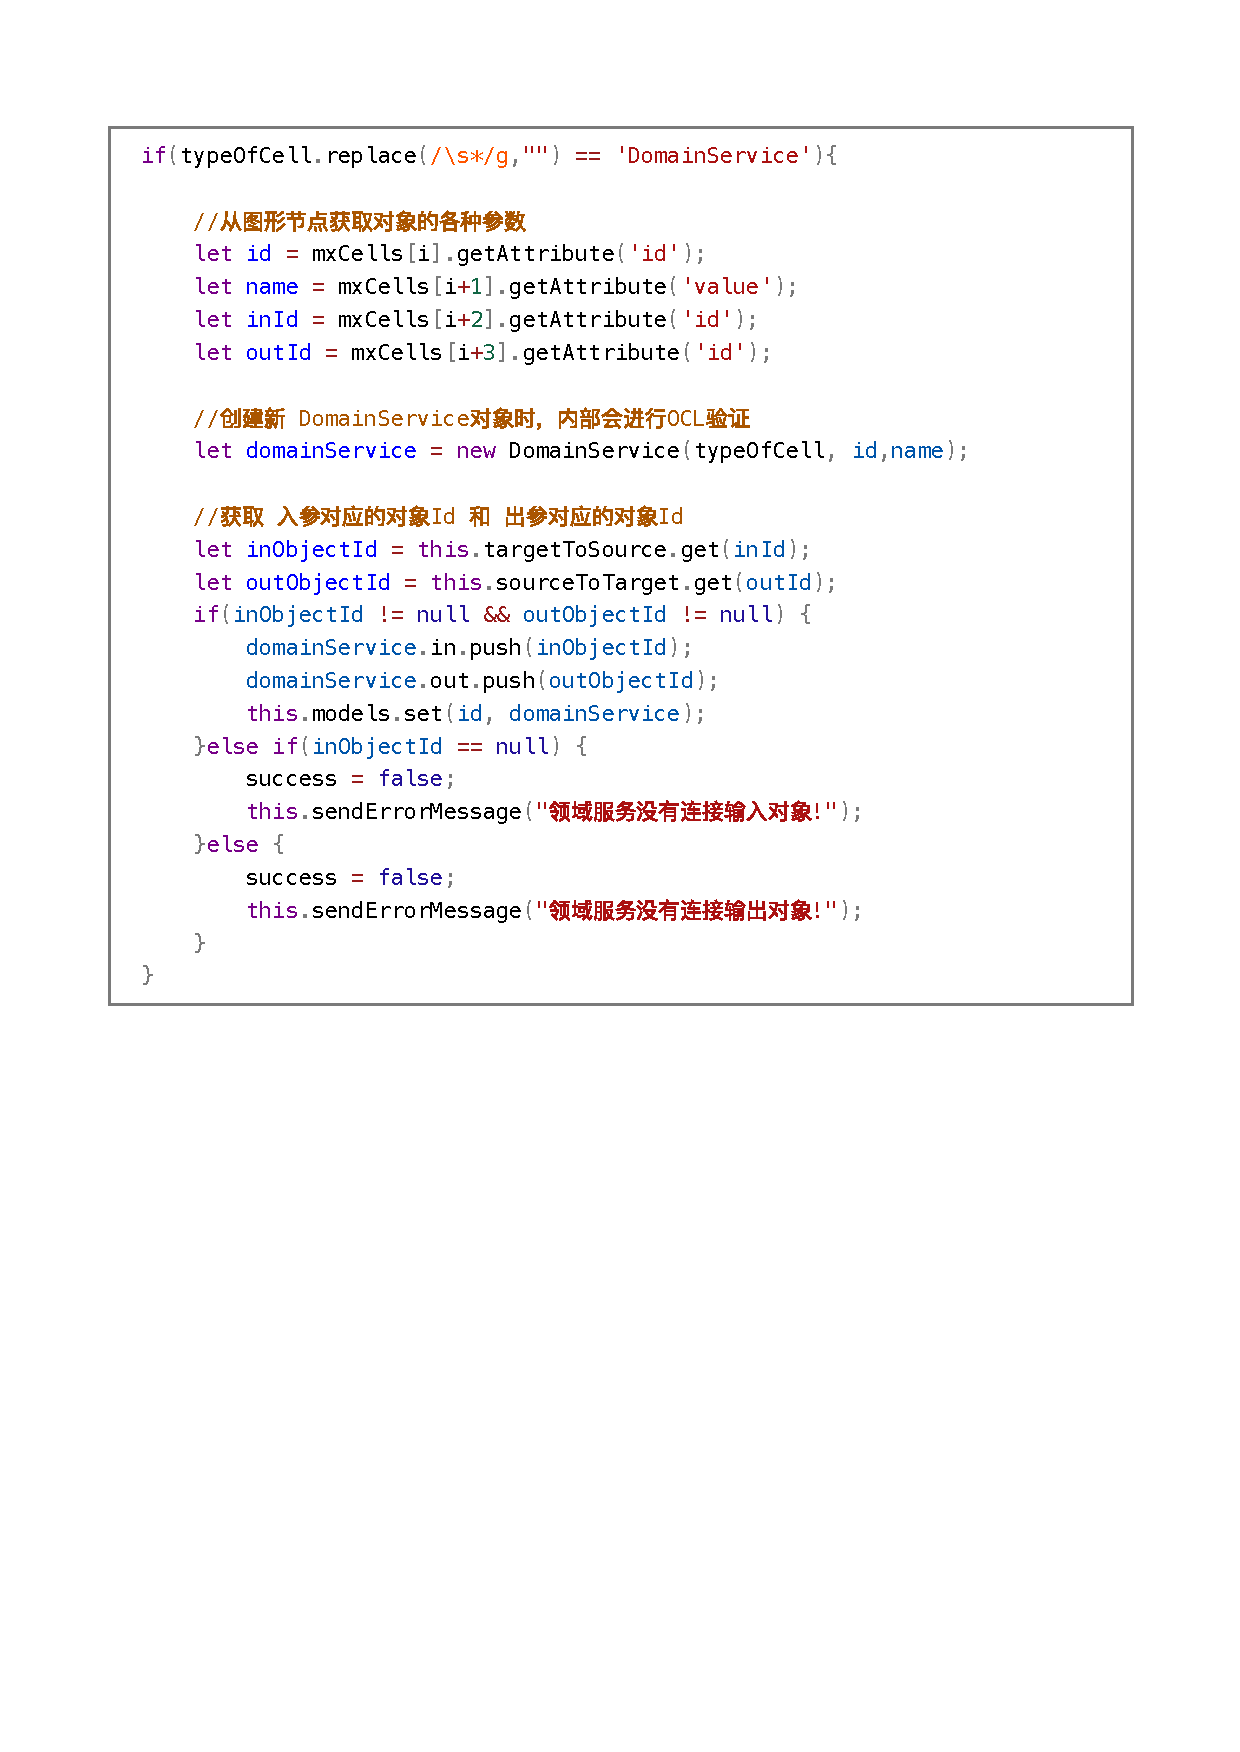
\includegraphics[width=0.8\textwidth]{FIGs/chapter4/validation.pdf} %中括号中的参数是设置图片充满文档的大小,你也可以使用小数来缩小图片的尺寸。
    \caption{模型校验部分实现代码} %caption是用来给图片加上图题的
    \label{validationCode} %这是添加标签,方便在文章中引用图片。
\end{figure}%figure环境


\subsection{模型存储与转化详细设计与实现}

本小节将介绍“模型存储与转化”模块的详细设计与实现。详细设计部分,
通过类图展现“模型存储与转化”模块的静态详细设计,
通过顺序图展现“模型存储与转化”模块的动态业务流程详细设计。
实现部分,通过部分核心功能实现代码进行展现。
“模型存储与转化”模块具体的设计如下:

\textbf{模型存储与转化类图}

“模型存储与转化”模块的类图如图\ref{classModelStorage}所示。
本工具提供对建模结果的存储与转化,由File类负责收集和组织图形化模式
的具体信息,可以直接在浏览器客户端导出建模结果的XML格式文件和图像格式文件,
也可以导入模型的XML文件,直接将模型绘制在画布上继续进行编辑;
当与后端进行通信时,会将模型信息抽象为Model类,由ModelRepository负责
模型的存储、修改、删除以及检索,
使用ElasticSearch提供的客户端进行持久化支持,
可以极大提升检索模型文件的效率。

\begin{figure}[!htbp] %figure环境,h默认参数是可以浮动,不是固定在当前位置。如果要不浮动,你就可以使用大写float宏包的H参数,固定图片在当前位置,禁止浮动。
    \centering %使图片居中显示
    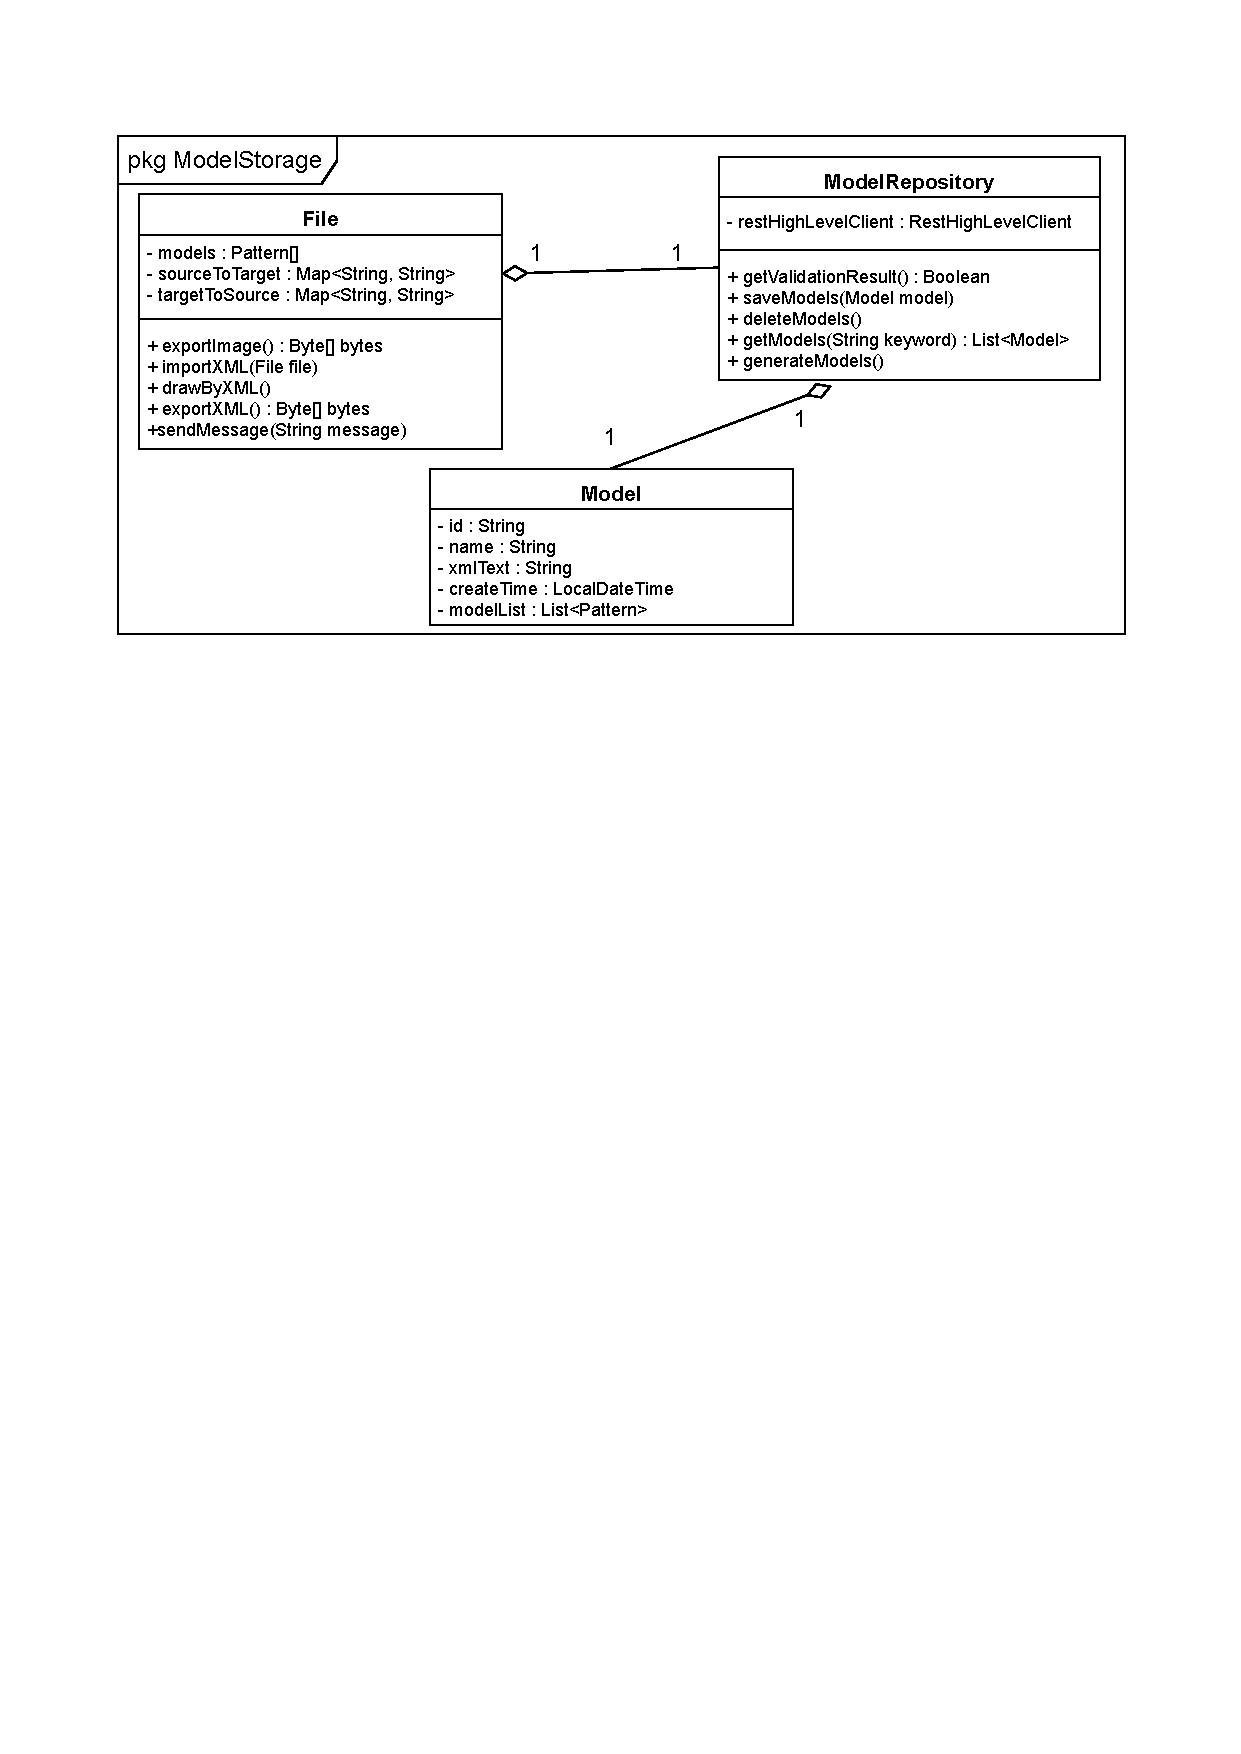
\includegraphics[width=0.8\textwidth]{FIGs/chapter4/classModelStorage1.pdf} %中括号中的参数是设置图片充满文档的大小,你也可以使用小数来缩小图片的尺寸。
    \caption{模型存储与转化类图} %caption是用来给图片加上图题的
    \label{classModelStorage} %这是添加标签,方便在文章中引用图片。
\end{figure}%figure环境

\newpage
\textbf{模型存储与转化顺序图}

“模型存储与转化”功能的示例过程如图\ref{sdModelStorage}所示。
开发人员或架构师使用浏览器客户端将XML模型文件导入画布,可以直接进行编辑,
编辑完成后,可以选择导出为XML文件或图像格式,
也可以将模型存储到数据库中并生成符合领域驱动设计规范的框架项目。

\begin{figure}[!htbp] %figure环境,h默认参数是可以浮动,不是固定在当前位置。如果要不浮动,你就可以使用大写float宏包的H参数,固定图片在当前位置,禁止浮动。
    \centering %使图片居中显示
    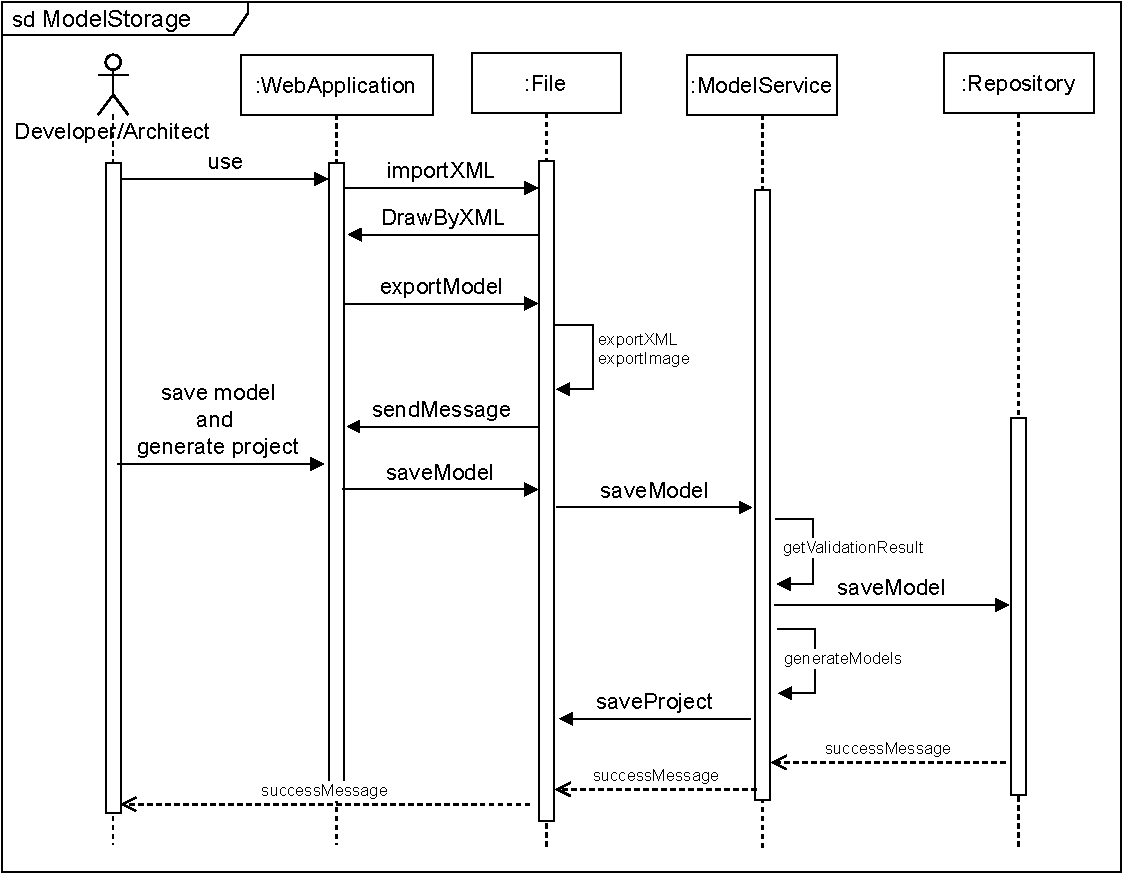
\includegraphics[width=0.8\textwidth]{FIGs/chapter4/sdModelStorage.pdf} %中括号中的参数是设置图片充满文档的大小,你也可以使用小数来缩小图片的尺寸。
    \caption{模型存储与转化顺序图} %caption是用来给图片加上图题的
    \label{sdModelStorage} %这是添加标签,方便在文章中引用图片。
\end{figure}%figure环境

\newpage
\textbf{模型存储部分实现代码}

如图\ref{saveModelcode}所示是“模型存储”部分实现代码。
主要描述将模型存储进ElasticSearch中的过程,
包括对模型对象的构建、存储格式的转化、发起存储请求与接收响应。


\begin{figure}[!htbp] %figure环境,h默认参数是可以浮动,不是固定在当前位置。如果要不浮动,你就可以使用大写float宏包的H参数,固定图片在当前位置,禁止浮动。
    \centering %使图片居中显示
    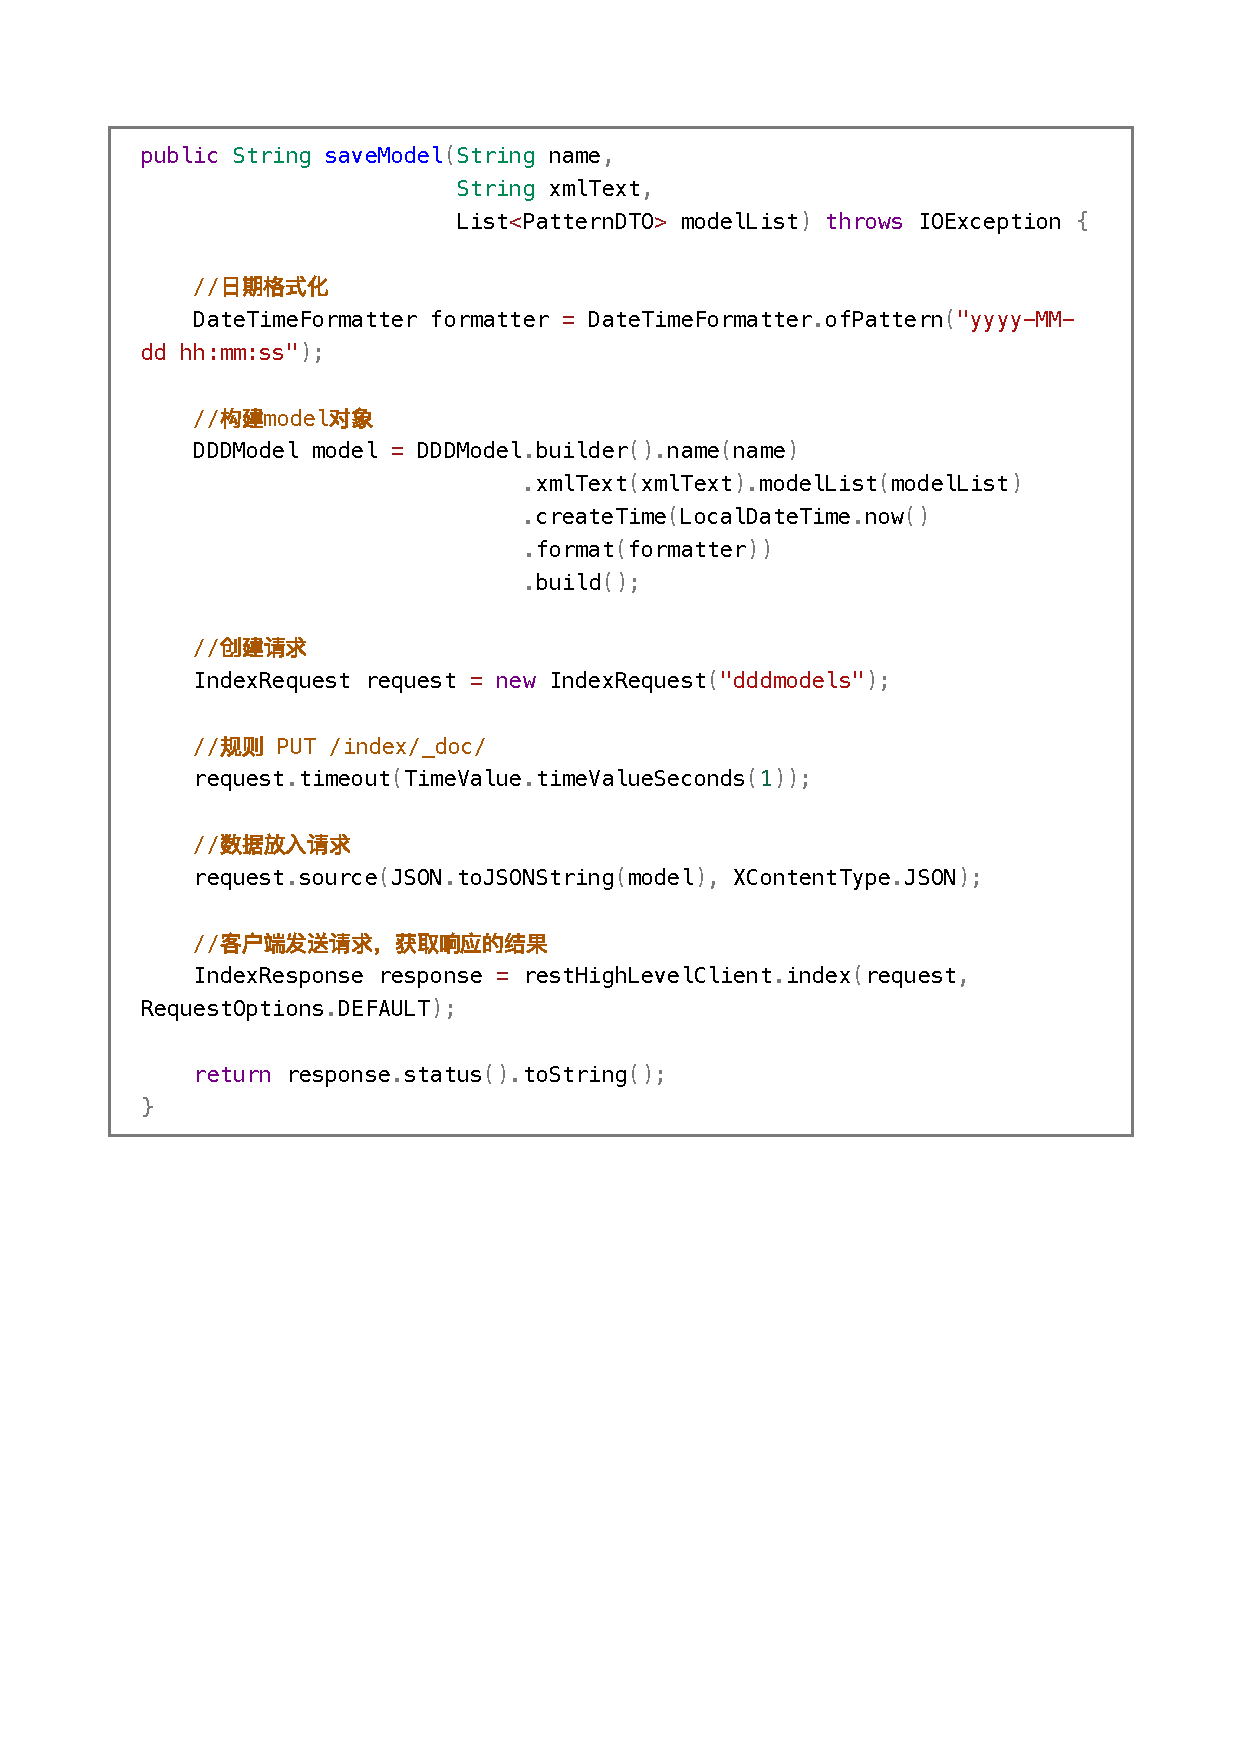
\includegraphics[width=0.8\textwidth]{FIGs/chapter4/saveModelcode.pdf} %中括号中的参数是设置图片充满文档的大小,你也可以使用小数来缩小图片的尺寸。
    \caption{模型存储部分实现代码} %caption是用来给图片加上图题的
    \label{saveModelcode} %这是添加标签,方便在文章中引用图片。
\end{figure}%figure环境

\section{本章小结}

本章介绍了建模支持工具的设计与实现。首先通过对建模场景中的用例分析,
获取具体需求,包括“可视化建模”、“模型校验”以及“模型存储与转化”三个主要模块。
然后对工具进行了功能性与非功能性需求的分析与展示,通过需求对工具进行总体设计
与详细设计。最后通过各模块功能类图、顺序图、功能算法逻辑和实现代码来展示工具的具体实现过程。

